\documentclass[preprint,review,12pt]{elsarticle}
\usepackage[T1]{fontenc}  
\usepackage[scaled=0.82]{beramono}  
\usepackage{microtype} 
\usepackage{amsmath}
\usepackage{subcaption}
\usepackage{float}
\usepackage{amsfonts}
\usepackage{mathtools}
\usepackage{bm}
\usepackage{slashed}
\usepackage{amssymb}
\usepackage{hyperref}
\usepackage{lineno}
\hypersetup{
    colorlinks=true,
    linkcolor=black,
    citecolor=black,
    urlcolor=black
}
\usepackage{nameref}
\usepackage{siunitx}
\usepackage{mhchem}
\usepackage{subcaption}
\usepackage[margin=2cm]{geometry}
\journal{Elsevier}
\DeclareMathOperator{\E}{E}
\DeclareMathOperator{\Var}{Var}
\begin{document}
\begin{frontmatter}
    \title{Single photoelectron charge spectra of MCP-PMTs coated by Atomic Layer Deposition}
    \author[a,b,c]{Jun Weng}
    \author[a,b,c]{Aiqiang Zhang}
    \author[d]{Qi Wu}
    \author[d]{Lishuang Ma}
    \author[d]{Sen Qian}
    \author[a,b,c]{Benda Xu\corref{cor1}}%
    \ead{orv@tsinghua.edu.cn}
    \author[a,b,c]{Zhe Wang}
    \author[a,b,c]{Shaomin Chen}

    \cortext[cor1]{Corresponding author}
    \affiliation[a]{
        organization={Department of Engineering Physics},
        addressline={Tsinghua University},
        city={Beijing},
        postcode={100084},
        country={China}}
    \affiliation[b]{
        organization={Center for High Energy Physics},
        addressline={Tsinghua University},
        city={Beijing},
        postcode={100084},
        country={China}}
    \affiliation[c]{
        organization={Key Laboratory of Particle \& Radiation Imaging (Tsinghua University)},
        addressline={Ministry of Education},
        country={China}}
    \affiliation[d]{
        organization={Institute of High Energy Physics},
        addressline={Chinese Academy of Sciences},
        city={Beijing},
        postcode={100049},
        country={China}
    }
    \begin{abstract}
        The atomic layer deposition~(ALD) coating lengthens the lifetimes of microchannel plates~(MCP), allowing them to act
        as the electron amplifier of photomultiplier tubes~(PMT).
        At the Jinping Neutrino Experiment~(JNE), the single electron response~(SER) charge distribution of
        the newly developed 8-inch MCP-PMT with ALD coating exhibits departures from the Gaussian distribution in large charge regions.
        To understand and model the mechanism of the large-charged SER,
        we design a voltage-division experiment to quantify the response of the MCP gains to the different energies of incident electrons.
        Combining with the Furman probabilistic model,
        this work first studies secondary electron emission~(SEE) in pulse mode
        and reproduces the SER charge spectra by introducing an additional MCP-surface amplification mode.
        Our results favor a Gamma-Tweedie mixture to describe the SER charge spectra of MCP-PMTs based on it.
    \end{abstract}
\end{frontmatter}
\linenumbers
\textbf{Keywords:} MCP-PMT, single electron response, secondary electron emission, Gamma distribution, Tweedie distribution
\section{Introduction}\label{sec:Introduction}
PMTs are vital devices in neutrino detection,
consisting of a photocathode, an electron multiplier, and an anode~\cite{1955Scintillation}.
Photons from a light source incident on the photocathode follow a Poisson process.
Some photons are converted to electrons via photoelectric effect
and the electrons are collected by the multiplier~\cite{2016Optimization},
which are Bernoulli selections with the probabilities being Quantum Efficiency~(QE) and Collection Efficiency~(CE).
The photoelectrons~(PEs, $n_{\mathrm{PE}}$) count in a specific time interval follows a Poisson distribution~\cite{1994Absolute}.

The electron amplification at the multiplier is based on the SEE~\cite{2021Summary} that
when an incident particle, electron or ion,
collides with or goes through a solid surface, one or more secondary electrons are emitted from the surface~\cite{2015Secondary}.
The average number of secondary electrons produced per incident particle is secondary-emission yield~(SEY, $\delta$),
and the energy distribution of the secondary electrons~(SES) is related to the initial energy of incident particle,
incident angle, target material, etc.~\cite{2002Probabilistic}.
Bruining~\cite{1938Secondary}, Ushio~\cite{1988Secondary}, and Jokela~\cite{2012Secondary}
conducted target-shooting experiments using electron guns,
and measured the SEY in current mode.
L. Olano measured the SES of Kapton, Teflon and Ultem by charging analysis and found the
energies are much smaller than that of the primary electrons~\cite{OLANO2020103456}.
Such results are then extrapolated to PMTs~\cite{2012An,2021Effects}.
Nevertheless, the low light intensity at which a PMT operates makes the incident electrons discrete.
Therefore, one should be more careful when extending the SEY from current mode to a single electron case which is pulse mode.

After amplification by the multiplier, one electron produces over $10^6$ electrons collected at the anode almost simultaneously.
The energies of photoelectrons when produced at the photocathode is only a few \si{eV}~\cite{Nathan1970TheED},
the initial energies of them are almost determined by the voltage difference
between the photocathode and the multiplier, therefore the gains for them are the same.
The output charge is often described by a Gaussian distribution in light of the central limit theorem of probability~\cite{1994Absolute}.
The probability density function~(PDF) for the total charge $Q$ of several PEs is,
\begin{equation}
    \begin{aligned}
        f(Q) & = P_{\pi}(n_{\mathrm{PE}};\lambda)\bigotimes f_{\mathcal{N}}(Q; n_{\mathrm{PE}}Q_1,n_{\mathrm{PE}}\sigma_1^2) \\
             & =\sum_{n_{\mathrm{PE}} = 0}^{\infty}\frac{\lambda^{n_{\mathrm{PE}}} e^{-\lambda}}{n_{\mathrm{PE}}!}
        \frac{1}{\sigma_1\sqrt{2\pi n_{\mathrm{PE}}}}\exp\left[-\frac{{(Q-n_{\mathrm{PE}}Q_1)}^2}{2n_{\mathrm{PE}}\sigma_1^2}\right]
    \end{aligned}
    \label{eq:sreal}
\end{equation}
where $\lambda$ is the average number of photoelectrons collected by the multiplier, $Q_1$ is the mean charge of a photoelectron,
and $\sigma_1$ is its standard deviation.\@
$P_\pi(n_{\mathrm{PE}};\lambda)$ and \(f_{\mathcal{N}}\) is are the PDFs of the Poisson distribution and Gaussian.
When $\lambda$ is less than 0.1,
the probability of two or more photoelectrons observed is less than one-tenth of the probability of one photoelectron.
The two visible peaks are attributed to the pedestal ($Q=0$) and the single photoelectron ($Q=Q_1$)~\cite{Xia_2015} as blue histogram shown in Fig~\ref{fig:spe_sreal}.
We study the SER charge spectrum divided by $Q_1$ as $Q/Q_1$ to align the gains of different PMTs.

Compared to a large-sized dynode-chain commonly used in PMT,
MCP-PMTs employ MCPs with the high gain and time resolution as electron multipliers~\cite{2021Summary},
and are currently in use or planned for particle physics experiments,
such as neutrino experiments like Jiangmen Underground Neutrino Observatory~(JUNO)~\cite{ZHU2020162002} and JNE~\cite{Zhang:2023ued},
collider experiments like Belle II TOP detector~\cite{MATSUOKA2014148} and PANDA DIRC Cherenkov detector at FAIR~\cite{KRAUSS2023168659},
and cosmic ray observation experiments like LHAASO~\cite{Cao2019UpgradingPT}.
Initially, MCP-PMTs were limited by lifetime issues
caused by the damage of MCP film layers~\cite{N2006Lifetime}.
A precise thin film deposition technique known as ALD~\cite{2012An}
has been applied in the fabrication of MCP-PMTs to solve the lifetime issues~\cite{Lehmann:2022ret}.
Lin Chen~et~al.~\cite{2016Optimization} indicated that using high SEY materials
such as \ce{Al2O3} and \ce{MgO} as ALD coating materials on the upper surface of MCP
can enhance the probability of collecting secondary electrons to improve CE
to nearly 100\% rather than being constrained by the MCP open area fraction.
This enhancement allows for increased gain, improved single electron resolution,
and a higher peak-to-valley ratio of MCP-PMTs~\cite{2021Effects}.

In the performance tests to evaluate MCP-PMT by JNE,
large charges are found in the SER charge spectrum of MCP-PMTs~\cite{Zhang:2023ued},
as shown in the red histogram in Fig~\ref{fig:spe_sreal}.
Similar significant charges have also been observed in the mass testing of PMTs in JUNO,
identified as the "long tail" in the SER charge distribution~\cite{JUNO:2022hlz}.
H.~Q.~Zhang~et~al.~\cite{2021Gain} used the SER charge model in Eq.~\eqref{eq:sreal} for large charges in JUNO
and recommended the calibration of gain.
A voltage division experiment reveals that
the charge gain obtained from incident low-energy electrons is significantly smaller than
that obtained from high-energy electrons, as measured by Yuzhen Yang et al.~\cite{2017MCP}.
Thus, the gains of the secondaries are different from the photoelectrons entering the channels directly.
The SER charge model in Eq.~\eqref{eq:sreal} is no longer sufficient to calibrate this type of PMT accurately.
A mechanism is necessary to explain the formation of these significant charges
and can thus develop an appropriate SER charge model for the MCP-PMT calibration.
\begin{figure}[ht]
    \centering
    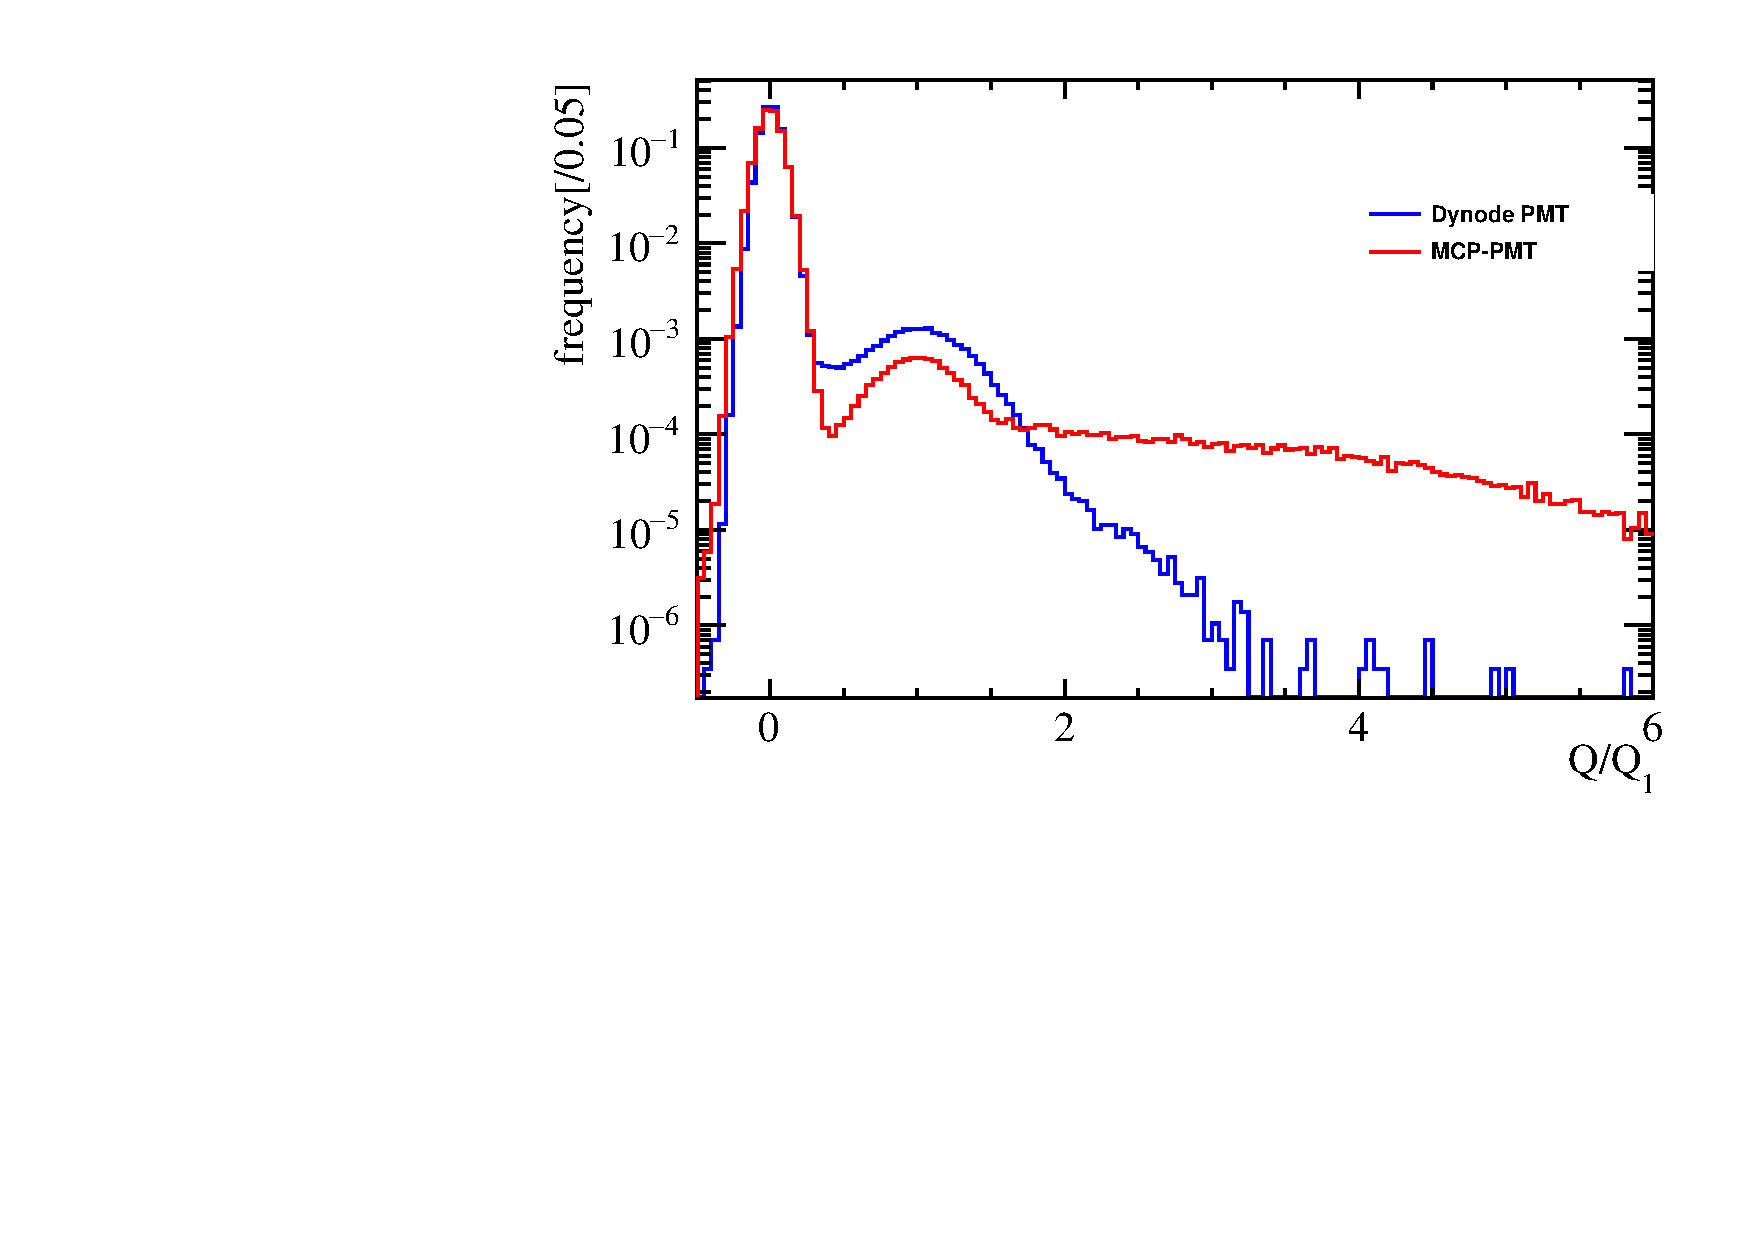
\includegraphics[width=0.7\textwidth]{pic/spe.pdf_total.pdf}
    \caption{The SER charge spectra of MCP-PMT PM2112-9089F~(red) and Dynode PMT~(blue).
        The blue histogram consists of the pedestal and the peak of $Q=Q_1$, while the red histogram includes additional large charges.}
    \label{fig:spe_sreal}
\end{figure}


In this paper, Gamma distribution is introduced in Sec.~\ref{gammapossion}.
In Sec.~\ref{sec:see}, a voltage-divided experiment is designed to measure the relationship
between the gains of MCP and the energies of incident electrons.
Considering the SEE model, we explain the cause of the large charges, and
measure the total SEY of \ce{Al2O3} and \ce{MgO} for the incident \SI{650}{eV} electrons.
Based on the explanation, a Gamma-Tweedie mixture is proposed for MCP-PMT in Sec.~\ref{sec:model}.
Discussion and conclusion are in Sec.~\ref{sec:discussion} and Sec.~\ref{sec:conclusion}.

\section{SER charge spectrum based on Gamma distribution}\label{gammapossion}
Instead of Gaussian containing a small nonphysical tail less than 0,
the charge distribution is parameterized with a Gamma distribution $\varGamma(\alpha, \beta)$ defined by a scale factor $\alpha$ and the rate fator $\beta$ as Eq.~\eqref{eq:gamma}:
\begin{equation}
    \label{eq:gamma}
    \begin{aligned}
        f_\Gamma(x ; \alpha, \beta) = \frac{x^{\alpha-1} e^{-\beta x} \beta^\alpha}{\Gamma(\alpha)} \quad \text { for } x>0 \quad \alpha, \beta>0 \\
    \end{aligned}
\end{equation}
where $\Gamma(\alpha)$ is the Gamma function.
A Gamma distribution uniquely determined by its expectation \(\frac{\alpha}{\beta}\) and variance \(\frac{\alpha}{\beta^2}\)
which can be converted into the mean and the variance of the Gaussian.

Every multiplication of electrons at the dynodes or MCP channels follows a Poisson distribution~\cite{branchandPoisson}.
A series of such multiplications forms a cascade Poisson distribution~\cite{1955Scintillation}.
It is a Galton-Watson branching process~\cite{Bartlett1963TheTO}
and difficult to perform analytical computations.
Breitenberger summaried and indicated that the shape of SER charge spectrum is between the Poisson distribution
and the Gaussian distribution~\cite{1955Scintillation}.
Prescott proposed to utilize a cascade Polya distribution to
characterize the electron multiplication in PMT
when considering the non-uniformity of the dynode surface~\cite{polya}.
Kalousis approximated the Polya distribution as a Gamma distribution to calibrate PMT
and achieved better calibration results than Gaussian model in Eq.~\eqref{eq:sreal}~\cite{2012Calibration,2020A}.
Similar to Eq.~\eqref{eq:sreal}, the SER charge spectrum based on the Gamma distribution is,
\begin{equation}
    \begin{aligned}
        f(Q) & = P_\pi(n_{\mathrm{PE}};\lambda)\bigotimes f_\Gamma(Q;n_{\mathrm{PE}}\alpha, \beta) \\
    \end{aligned}
    \label{eq:Gamma}
\end{equation}
where \(\frac{\alpha}{\beta}=Q_1\) and \(\frac{\alpha}{\beta^2}=\sigma_1^2\).
\section{Explanation for large charges based on secondary electron emission}\label{sec:see}

\subsection{The structure of MCP-PMT}\label{subsec:structure}
MCP-PMT deploies two pieces of MCPs as the electron multiplier.
The photoelectrons are amplified by MCP through a branching process described in Sec.~\ref{gammapossion}
and a large number of electrons produced at the end of the MCP reach the anode to form electrical signals~\cite{2013Photodetectors}.

\begin{figure}[H]
    \centering
    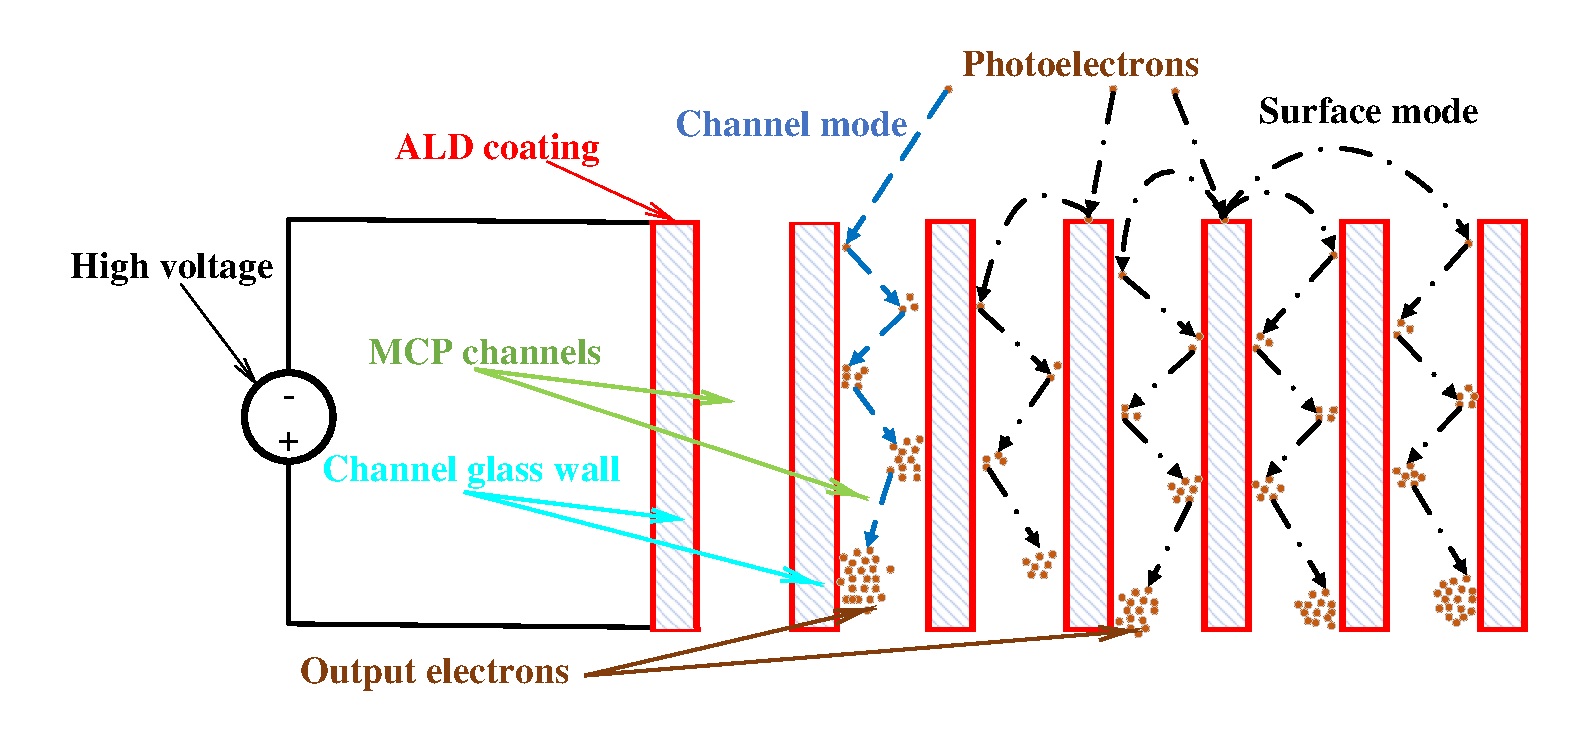
\includegraphics[width=0.7\textwidth]{pic/mcp.pdf}
    \caption{The photoelectrons directly enter the channels~(channel mode) or hit the upper surface producing secondary electrons
        which enter the channels later~(surface mode)~\cite{2016Optimization}. After entering the MCP channel, the electron collides
        with the channel wall for many times and is amplified in a series of such multiplications~\cite{1955Scintillation}.}\label{fig:MCP}
    \label{fig:mcp_modes}
\end{figure}

Besides, the secondary electrons from the upper surface of MCP can also enter the MCP channels for multiplication
under the influence of electric field.\@
Two independent mode dominate the amplification process as shown in Fig.~\ref{fig:mcp_modes}.
The \textit{channel mode} is that photoelectrons directly enter the channels
and the other is the \textit{surface mode} that secondary electrons from the upper surface enter the channels.
The selection of these two modes follows Bernoulli distribution~\cite{1955Scintillation}.

\subsection{Furman probabilistic model}\label{subsec:fuman}
The Furman probabilistic model~(Furman model)~\cite{2002Probabilistic}
is a theoretical framework employed to elucidate the phenomenon of SEE from solid surfaces.
This model incorporates the statistical nature of the SEE process
by considering the probability distribution governing the number of secondary electrons emitted per incident primary electron.
Each emission event of a secondary electron is regarded as an independent occurrence,
with its energy following the distribution contingent upon material properties and the primary energy.

In Furman model, the SES can be represented as $d\delta/dE$,
where $E$ is the energy of secondary electron.
There are three kinds of secondary electrons emitted.
The first kind is the back-scattered electron that secondary electrons are emitted by elastic scattering on the surface of the target material.
The SES is defined as Eq.~\eqref{eq:backscatter},
where $\delta_{\mathrm{bs}}$ is the yield of back-scatter electron,
$\theta(E)$ function ensures the $E<E_0$,
$E_0$ is the incident energy of the primary electron,
$\theta_0$ is the incident angle,
and $\sigma_{\mathrm{bs}}$ is an adjustable standard deviation.
\begin{equation}
    \label{eq:backscatter}
    \begin{aligned}
         & \frac{\delta_{\mathrm{bs}}}{dE} =\theta(E) \theta\left(E_0-E\right) \delta_{\mathrm{bs}}\left(E_0, \theta_0\right)
        \frac{2 \exp \left(-\left(E-E_0\right)^2 / 2 \sigma_{\mathrm{bs}}^2\right)}{\sqrt{2 \pi} \sigma_{\mathrm{bs}}
        \operatorname{erf}\left(E_0 / \sqrt{2} \sigma_{\mathrm{bs}}\right)}                                                   \\
    \end{aligned}
\end{equation}

The second kind is the rediffused electron that secondary electrons are generated by atomic scattering after electrons enter the target material.
The SES of rediffused electrons is defined as Eq.~\eqref{eq:rediffused},
where $\delta_{\mathrm{rd}}$ the yield of rediffused electron,
and $q$ is an adjustable parameter.
\begin{equation}
    \label{eq:rediffused}
    \begin{aligned}
         & \frac{\delta_{\mathrm{rd}}}{dE} =\theta(E) \theta\left(E_0-E\right) \delta_{\mathrm{rd}}\left(E_0, \theta_0\right) \frac{(q+1) E^q}{E_0^{q+1}} \\
    \end{aligned}
\end{equation}

The final and most important kind is the true-secondary electrons.
Upon penetration of electrons into the target material more deeply, intricate physical processes ensue,
resulting in the generation of one or more secondary electrons.
This is the only one process which occurs with the multiplication of electrons.
The SES of true-secondary electrons is defined as Eq.~\eqref{eq:true}.
\begin{equation}
    \label{eq:true}
    \begin{aligned}
        \frac{d \delta_{\mathrm{ts}}}{d E}=  \sum_{n=1}^{\infty}
        \frac{n P_{\mathrm{n, ts}}\left(E_0\right)
        \left(E / \epsilon_{\mathrm{n}}\right)^{p_{\mathrm{n}}-1} e^{-E / \epsilon_{\mathrm{n}}}}
        {\epsilon_{\mathrm{n}} \Gamma\left(p_{\mathrm{n}}\right) P\left(n p_{\mathrm{n}}, E_0 / \epsilon_{\mathrm{n}}\right)}
        \times P\left[(n-1) p_{\mathrm{n}},\left(E_0-E\right) / \epsilon_{\mathrm{n}}\right]
    \end{aligned}
\end{equation}
where $\delta_{\mathrm{ts}}$
is the yield of true-secondary electrons,
$\epsilon_{\mathrm{n}}$ and $p_{\mathrm{n}}$ are greater than 0 as phenomenological parameters,
and $P(z,x)$ is the normalized incomplete gamma function satisfying $P(0,x)=1$.
The number of true-secondary electrons is $n$ following Poisson distribution $n\sim \mathrm{\pi}(\delta_{\mathrm{ts}})$,
$P_{\mathrm{n, ts}}$ is the probability for emitting $n$ true-secondary electrons
defined in Eq.~\eqref{eq:pnts}~\cite{2002Probabilistic}.
\begin{equation}
    \label{eq:pnts}
    P_{\mathrm{n, ts}}=P(n;\delta_{\mathrm{ts}}) = \frac{\delta_{\mathrm{ts}}^{n}}{n!}e^{-\delta_{\mathrm{ts}}}
\end{equation}

The following parameters are taken as
$\delta_{\mathrm{bs}}=0.1$, $\delta_{\mathrm{rd}}=1$, $\delta_{\mathrm{ts}}=5$~\cite{2021Effects},
$\theta_0=0$ and $E_0=$\SI{650}{eV},
and the total SES is
$f_\mathrm{SES}(E) = \frac{d\delta}{dE}=\frac{\delta_{\mathrm{bs}}}{dE}+\frac{\delta_{\mathrm{rd}}}{dE}+\frac{\delta_{\mathrm{ts}}}{dE}$
as shown in Fig.~\ref{fig:SES}.

\begin{figure}[ht]
    \centering
    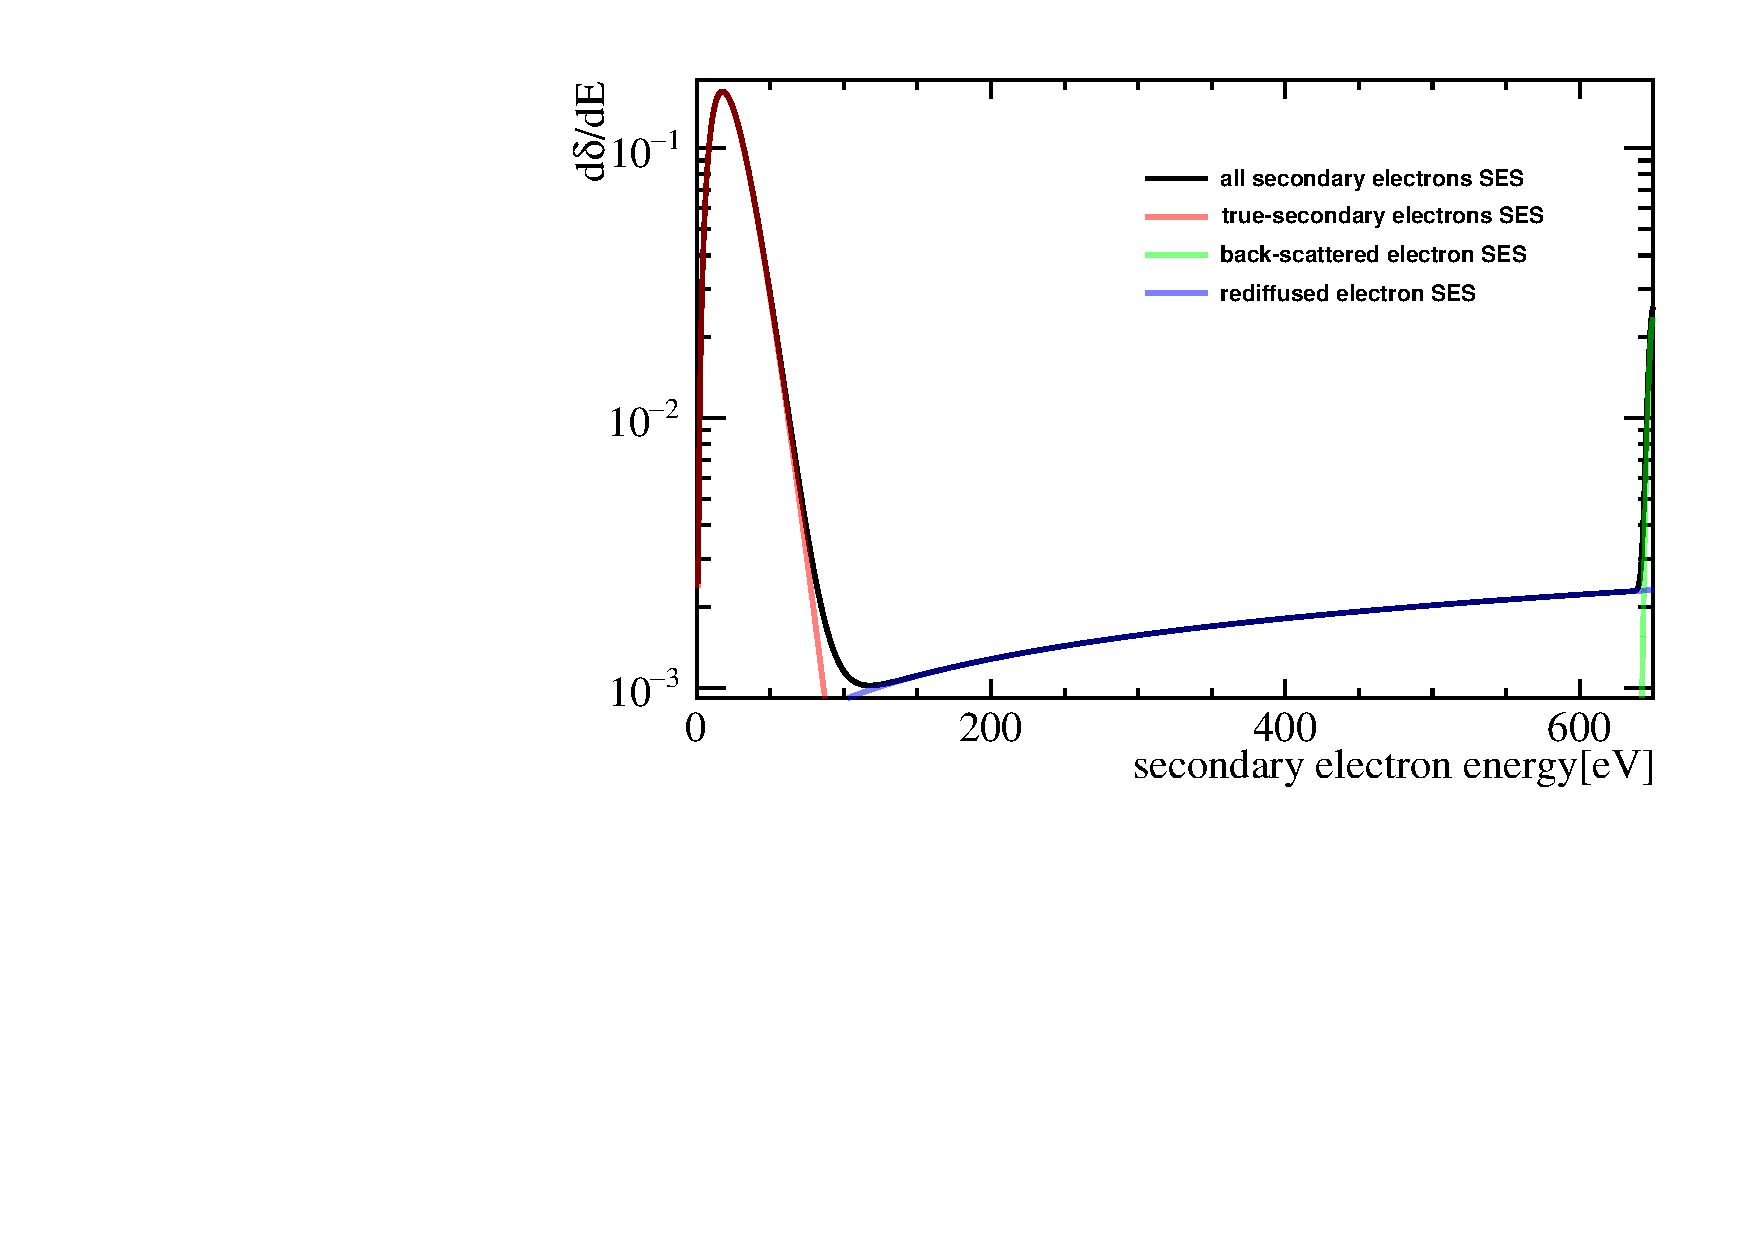
\includegraphics[width=0.6\textwidth]{pic/SES.pdf}
    \caption{When primary energy is \SI{650}{eV},
        the red line represents $d\delta_{\mathrm{bs}}/dE$,
        the blue line represents $d\delta_{\mathrm{rd}}/dE$,
        the green line represents $d\delta_{\mathrm{ts}}/dE$,
        and the black one is $d\delta/dE$.}
    \label{fig:SES}
\end{figure}


\subsection{Voltage-division Experiment}\label{sec:gain}
From Sec.~\ref{subsec:fuman} and as shown in Fig.~\ref{fig:SES},
secondary electrons have lower energies and usually less than \SI{100}{eV} when incident energy is \SI{650}{eV}.
When the primary energy is below \SI{100}{eV}, the SEY is much smaller than which at \SI{650}{eV}~\cite{2012An}.
Thus, the gain of single secondary electron is not the same as the photoelectrons directly entering the channels.
A voltage-division experiment is designed to measure the relationship
between the gains of MCP and the energies of electrons entering the MCP channels.

\subsubsection{Experimental setup}
The energy of the photoelectron arriving at the MCP is almost determined by the voltage difference
between the photocathode and the MCP, based on which we can control the energy of the electrons by adjusting the voltage.
As shown in the Fig.~\ref{fig:setup}, a positive and a negative high voltage supplies are used.
A high sampling rate oscilloscope is used to capture all the waveforms.

As shown in Fig.~\ref{fig:circuit}, an adjustable high voltage between the photocathode and $\mathrm{M}1$ the upper surface of the first MCP
is provided by the negative high voltage power supply.
The positive high voltage power supply delivers 4 consistent voltages to the two MCPs
after being divided by resistors as shown in Fig.~\ref{fig:setup} following the voltage divider designed in~\cite{Luo:2023jdf}.
There is a stable voltage difference between the two MCPs difined as the gap voltage~\cite{2017MCP}.
With this experimental setup,
simultaneously adjusting the electron incident energy
and keeping the voltage division of the MCPs stability are achieved.
This can also be accomplished by using more power supplies~\cite{2017MCP}
which is harder to operate but easier to change the voltage differences of MCPs.
\begin{figure}[ht]
    \centering
    \begin{subfigure}{\textwidth}
        \centering
        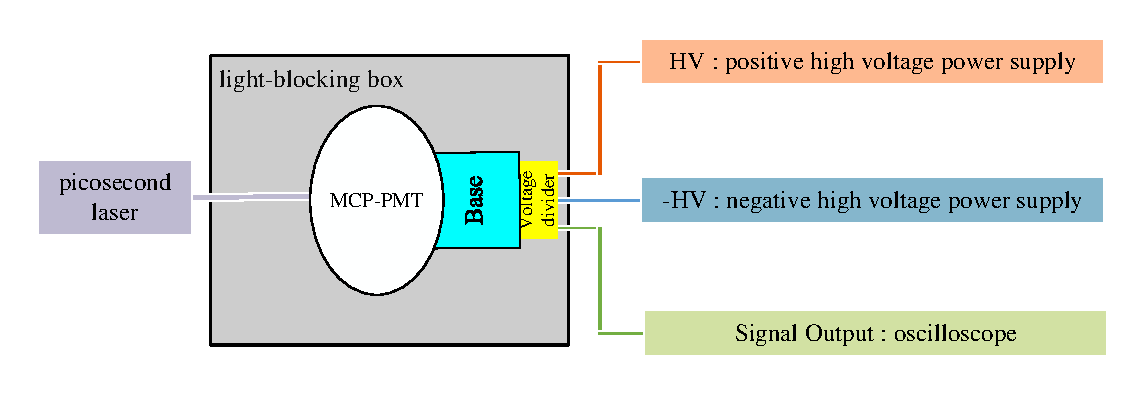
\includegraphics[width=0.7\linewidth]{pic/setup.pdf}
        \caption{}
        \label{fig:setup}
    \end{subfigure}
    \vspace{0.5cm}
    \begin{subfigure}{\textwidth}
        \centering
        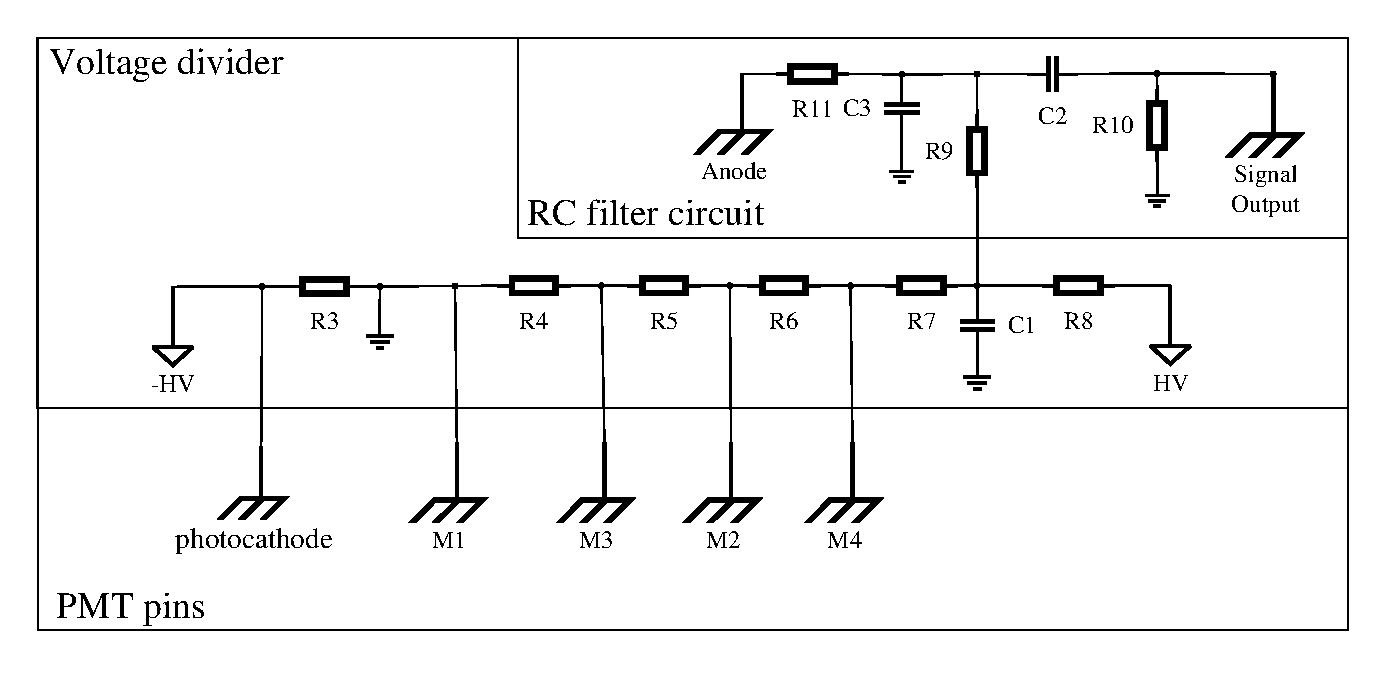
\includegraphics[width=0.7\linewidth]{pic/circuit.pdf}
        \caption{}
        \label{fig:circuit}
    \end{subfigure}
    \caption{Experimental setup and the circuit of voltage divider.
        The plot~\subref{fig:setup} is schematic diagram of the experimental setup:
        simultaneously supply positive and negative high voltages to the MCP-PMT,
        and capture the output waveforms using an oscilloscope.
        The plot~\subref{fig:circuit} is the experimental circuit diagram:
        supply the photocathode with the negative high voltage,
        supply the two MCPs with the positive high voltage,
        and use an RC filtering and shaping circuit
        to convert the amplified electrical signal into waveforms output.
        $\mathrm{M}1$, $\mathrm{M}3$ are the upper surfaces of MCPs
        and $\mathrm{M}2$, $\mathrm{M}4$ are the lower surfaces.
        The gap voltage is between $\mathrm{M}2$ and $\mathrm{M}3$.}
    \label{fig:mainfig}
\end{figure}

\subsubsection{Relationship of gain and incident energy}
A new waveform analysis method named fast stochastic matching pursuit~(FSMP)~\cite{Xu_2022}
utilizing Markov Chain Monte Carlo is employed. With the best accurate time and intensity resolution,
FSMP provides more precise measurements of SER charge spectrum.

To exclude the influence of the surface mode, we conducted the same test on MCP-PMTs with and without ALD coating.
\begin{figure}[ht]
    \centering
    \begin{subfigure}[b]{0.48\textwidth}
        \centering
        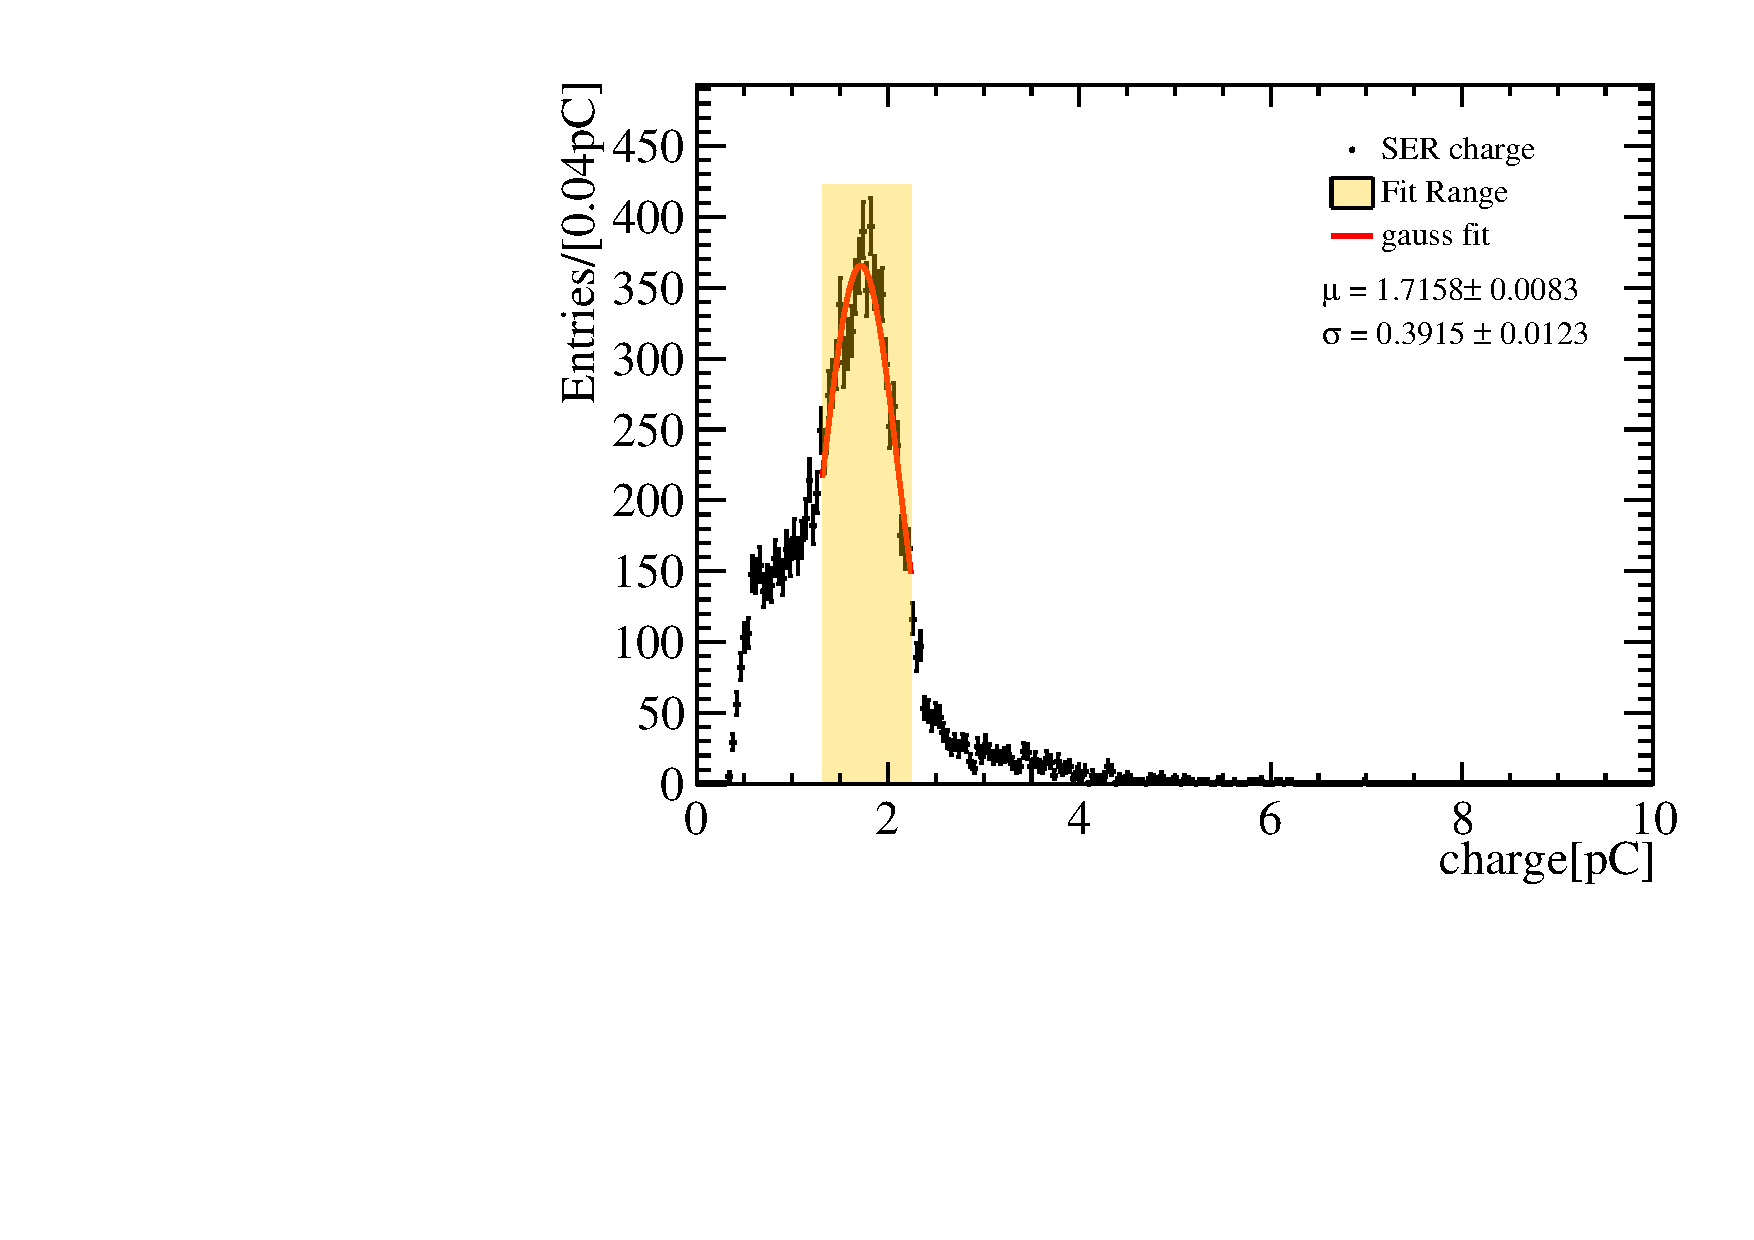
\includegraphics[width=\textwidth]{pic/SER_noALD.pdf}
        \caption{}
        \label{fig:gain_noald}
    \end{subfigure}
    \hfill
    \begin{subfigure}[b]{0.48\textwidth}
        \centering
        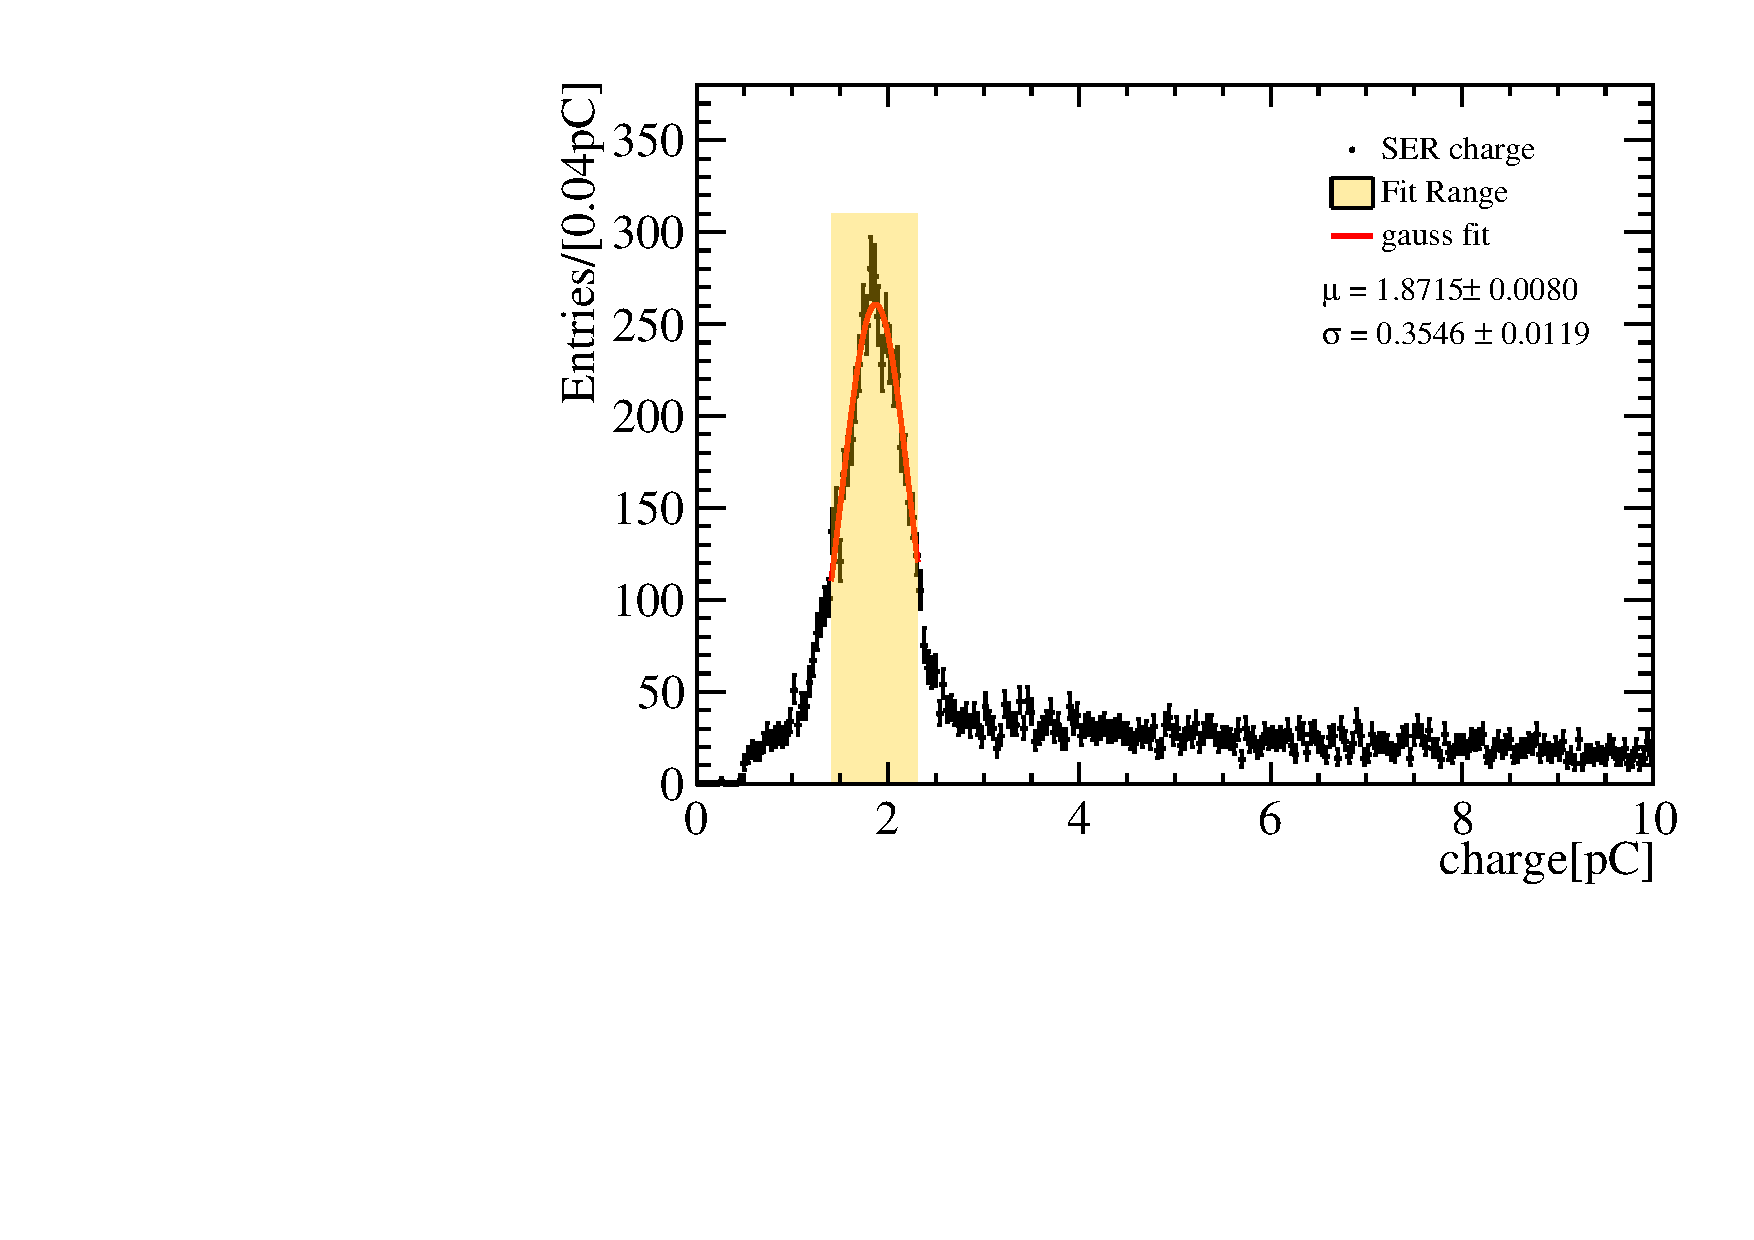
\includegraphics[width=\textwidth]{pic/SER_ALD.pdf}
        \caption{}
        \label{fig:gain_ald}
    \end{subfigure}
    \caption{The plot~\subref{fig:gain_noald} displays the fit of the charge spectrum of the MCP-PMT without ALD coating,
        while the plot~\subref{fig:gain_ald} shows the fit with ALD coating.
        We observed that the plot~\subref{fig:gain_noald} does not exhibit large charges.}
    \label{fig:gain_fit}
\end{figure}
The $\mu$ and $\sigma$ are calculated for every initial energy
by fitting the main peak of SER charge spectra with Gaussian distribution as shown in Fig.~\ref{fig:gain_fit},
$g_{\mathrm{\mu,\sigma}}(E)$ is the function to describe the relationship between gains and electron energies as shown in Fig.~\ref{fig:gaintest}.

\begin{figure}[ht]
    \centering
    \begin{subfigure}[b]{0.48\textwidth}
        \centering
        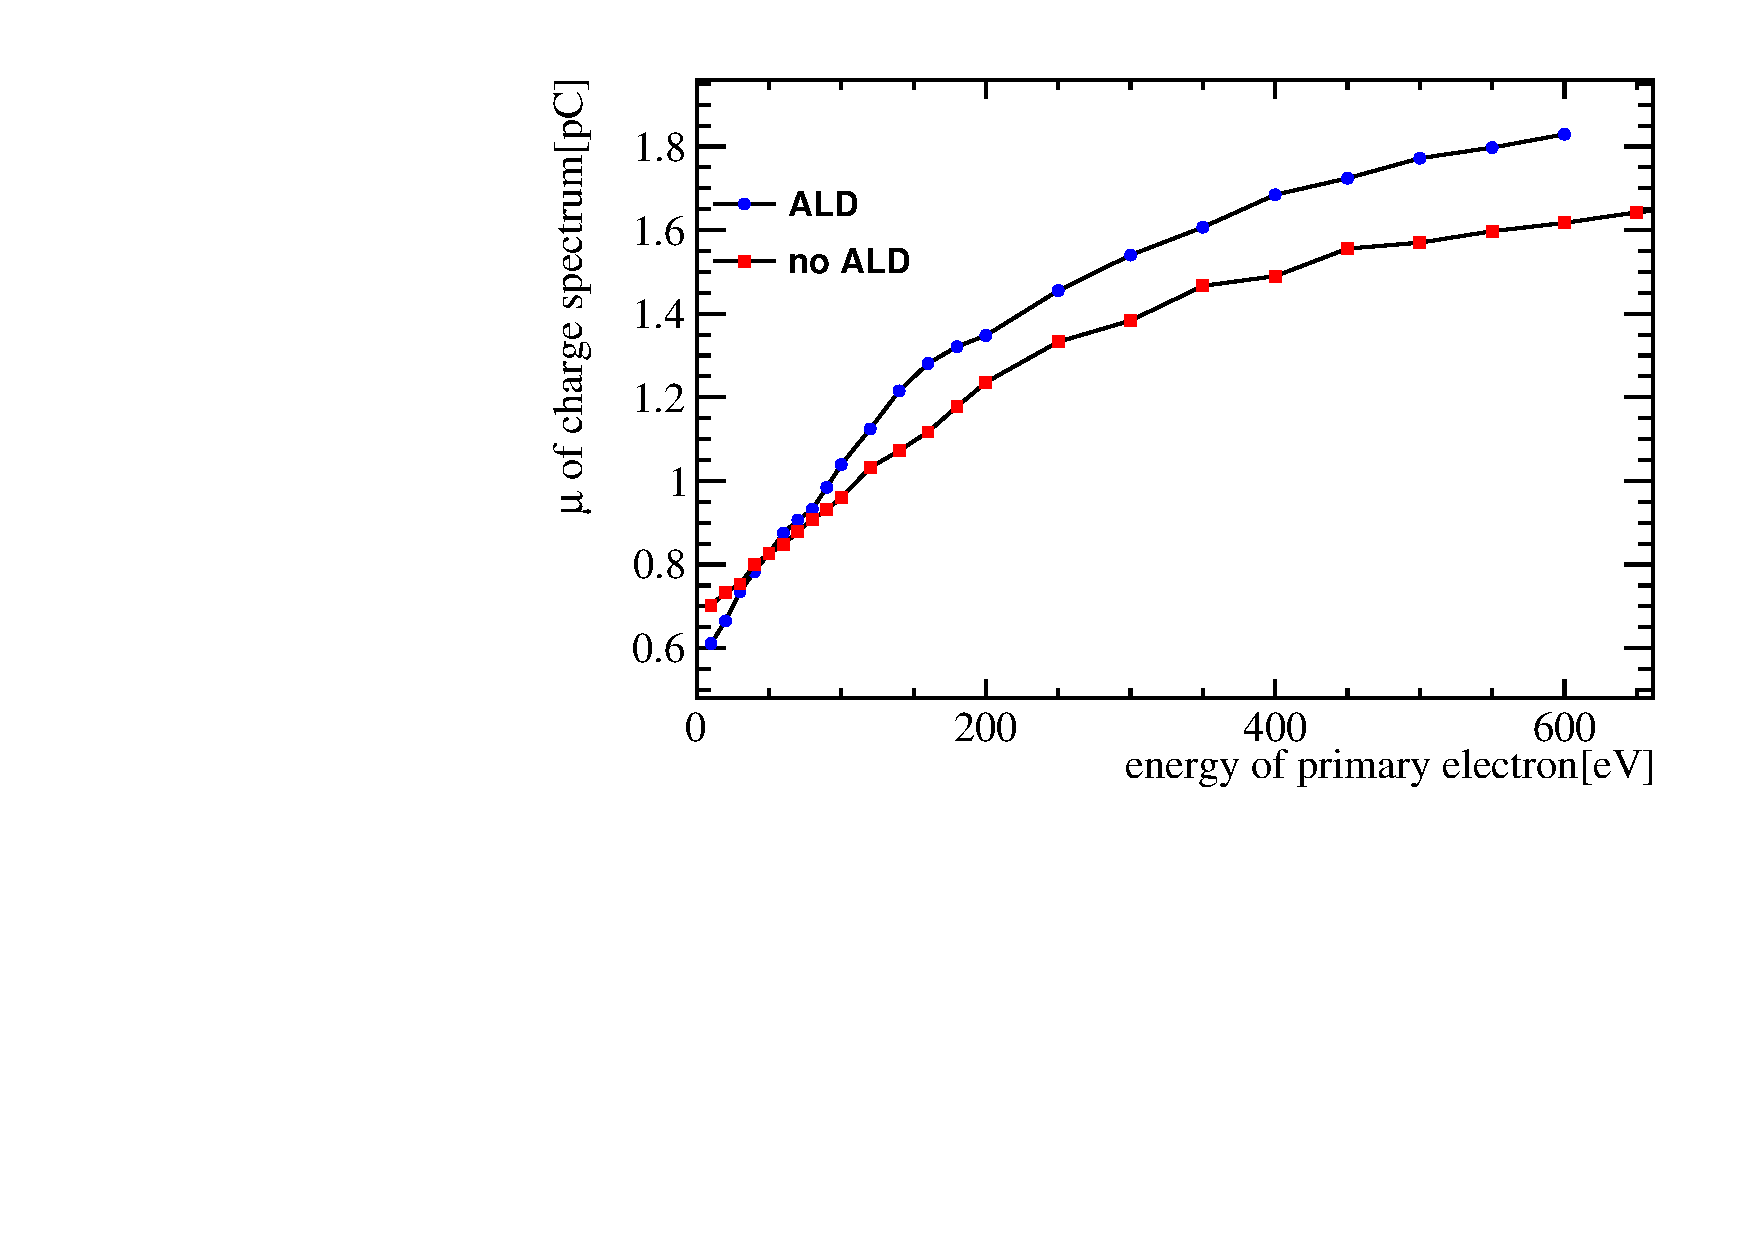
\includegraphics[width=\textwidth]{pic/gain.h5_mu.pdf}
        \caption{}
        \label{fig:gain}
    \end{subfigure}
    \hfill
    \begin{subfigure}[b]{0.48\textwidth}
        \centering
        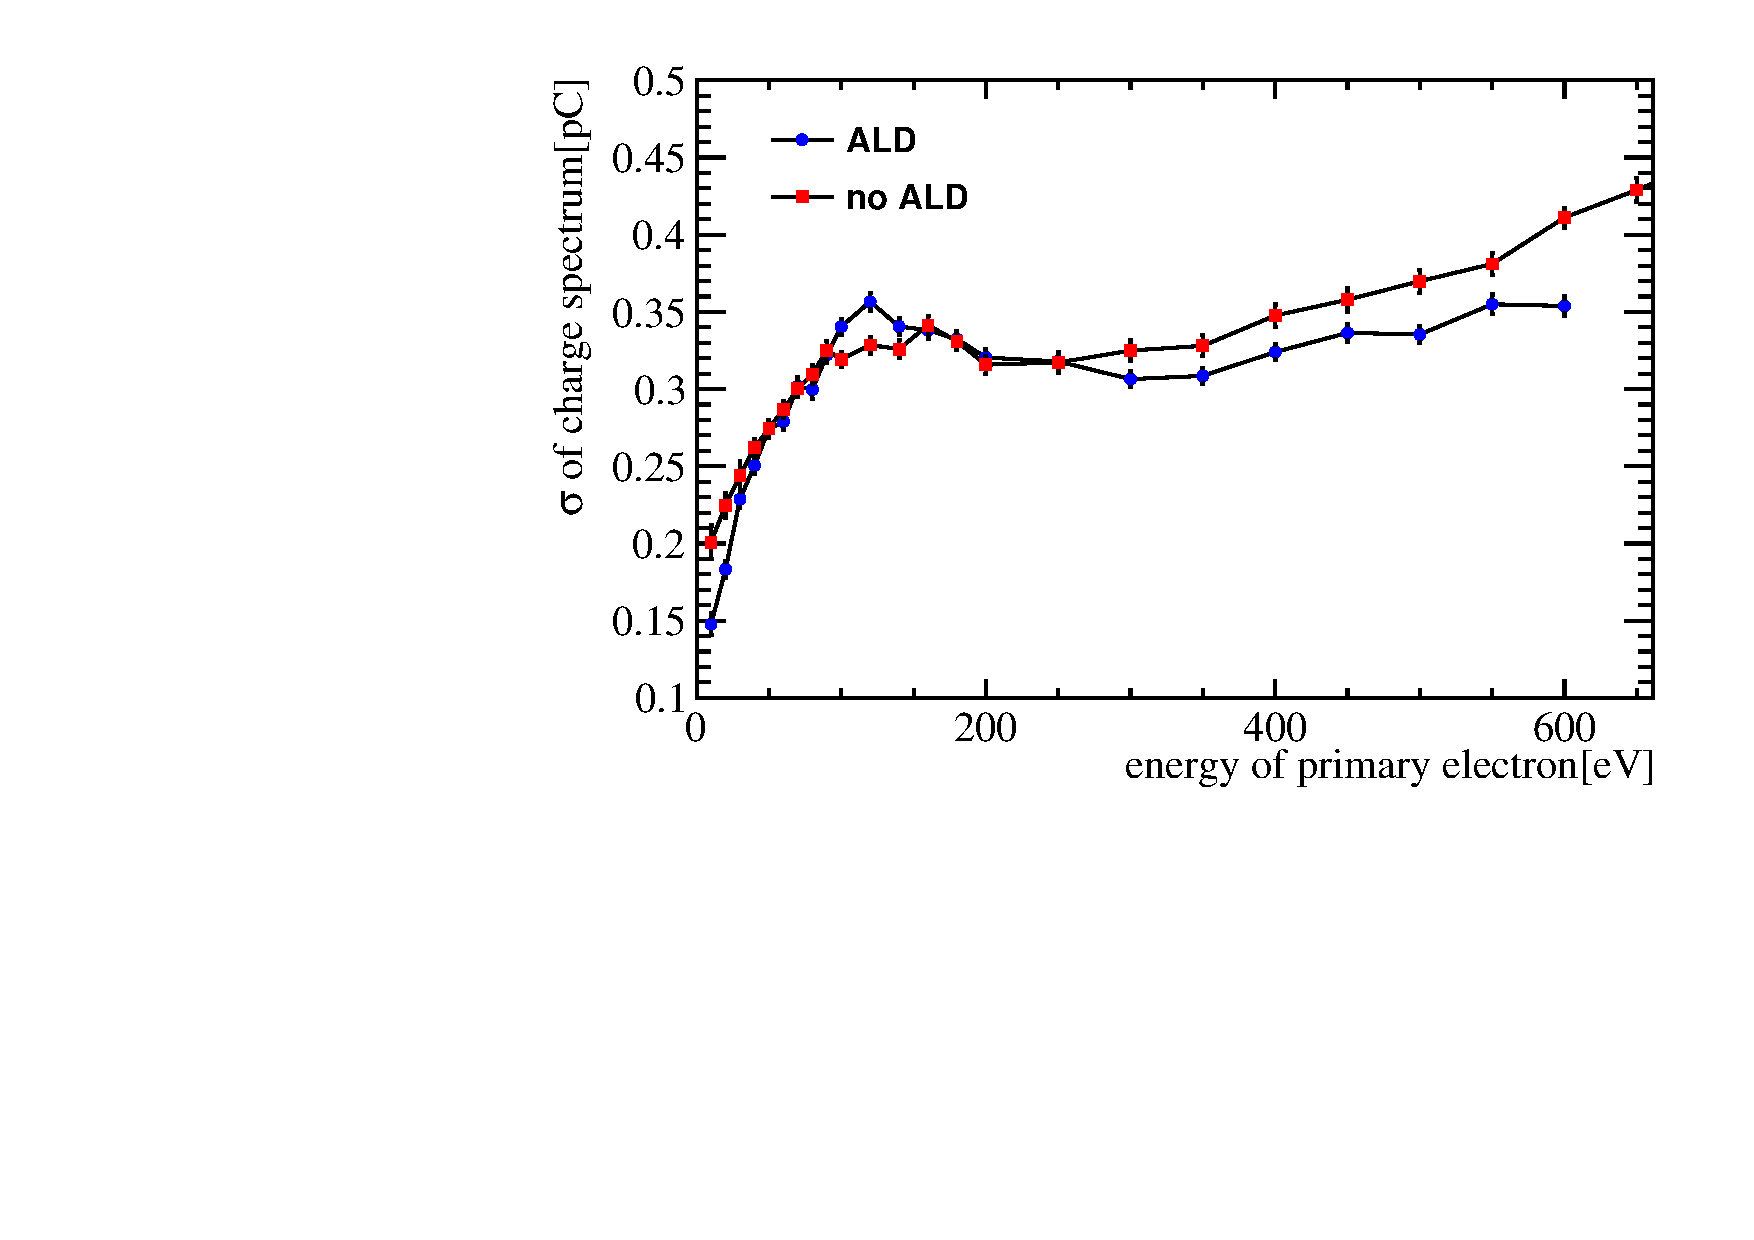
\includegraphics[width=\textwidth]{pic/gain.h5_sigma.pdf}
        \caption{}
        \label{fig:sigma}
    \end{subfigure}
    \caption{The plot~\subref{fig:gain} shows that the mean increases as initial electron energy increases,
        and the plot~\subref{fig:sigma} shows the variance changes with energy.
        MCP-PMT with ALD coating~(the red line) shows a similar variation trend to the one without ALD coating~(the blue line).}
    \label{fig:gaintest}
\end{figure}

When the electron energy is less than \SI{400}{eV} , the gain rapidly increases with the electron energy.
As the electron energy reaches \SI{400}{eV}, the gain gradually stabilizes.
Similar results are reported in~\cite{2017MCP}.
The gains for the low-energy secondary electrons
from the surface mode are lower than that from channel mode.

The charge responses of electrons with different energies are superimposed
according to the SES to obtain the charge response of the surface mode.

\subsection{Monte Carlo calculation}\label{sec:convolution}
Note the probability of electrons directly entering the channel and hitting on the MCP upper surface as $p$ and $1-p$.
Considering that the number of secondary electrons~$n_{\mathrm{se}}$ may exceed 1,
The SER charge can be described as Eq.~\eqref{eq:convolution},
\begin{equation}
    \label{eq:convolution}
    \begin{aligned}
        Q_{\mathrm{MCP-PMT}} & = p\times Q_{\mathrm{channel}}+(1-p)\times Q_{\mathrm{surface}}                                                            \\
                             & = p\times Q_{\mathrm{channel}}+(1-p)\times \frac{\int_0^{E_0}G(E)f_{\mathrm{SES}}(E)dE}{\int_0^{E_0}f_{\mathrm{SES}}(E)dE} \\
    \end{aligned}
\end{equation}
where $Q_{\mathrm{MCP-PMT}}$ is the SER charge distribution of MCP-PMT,
$Q_{\mathrm{channel}}$ and $Q_{\mathrm{surface}}$ are the charge distributions of the charge mode and the surface mode,
and $G(E)$ whose parameters are taken from $g_{\mathrm{\mu,\sigma}}$ is the charge distribution when incident energy is $E$.
The SER charge distribution is simulated using Monte Carlo method~\cite{1951Various} as shown in Fig.~\ref{fig:process}.
The probabilities of the three processes are approximated by the relative amounts of the yields.
For true-secondary electrons, their number $n$ is given by Poisson sampling and the sum of the sampled $n$ charges
serves as the output charge.
\begin{figure}[ht]
    \centering
    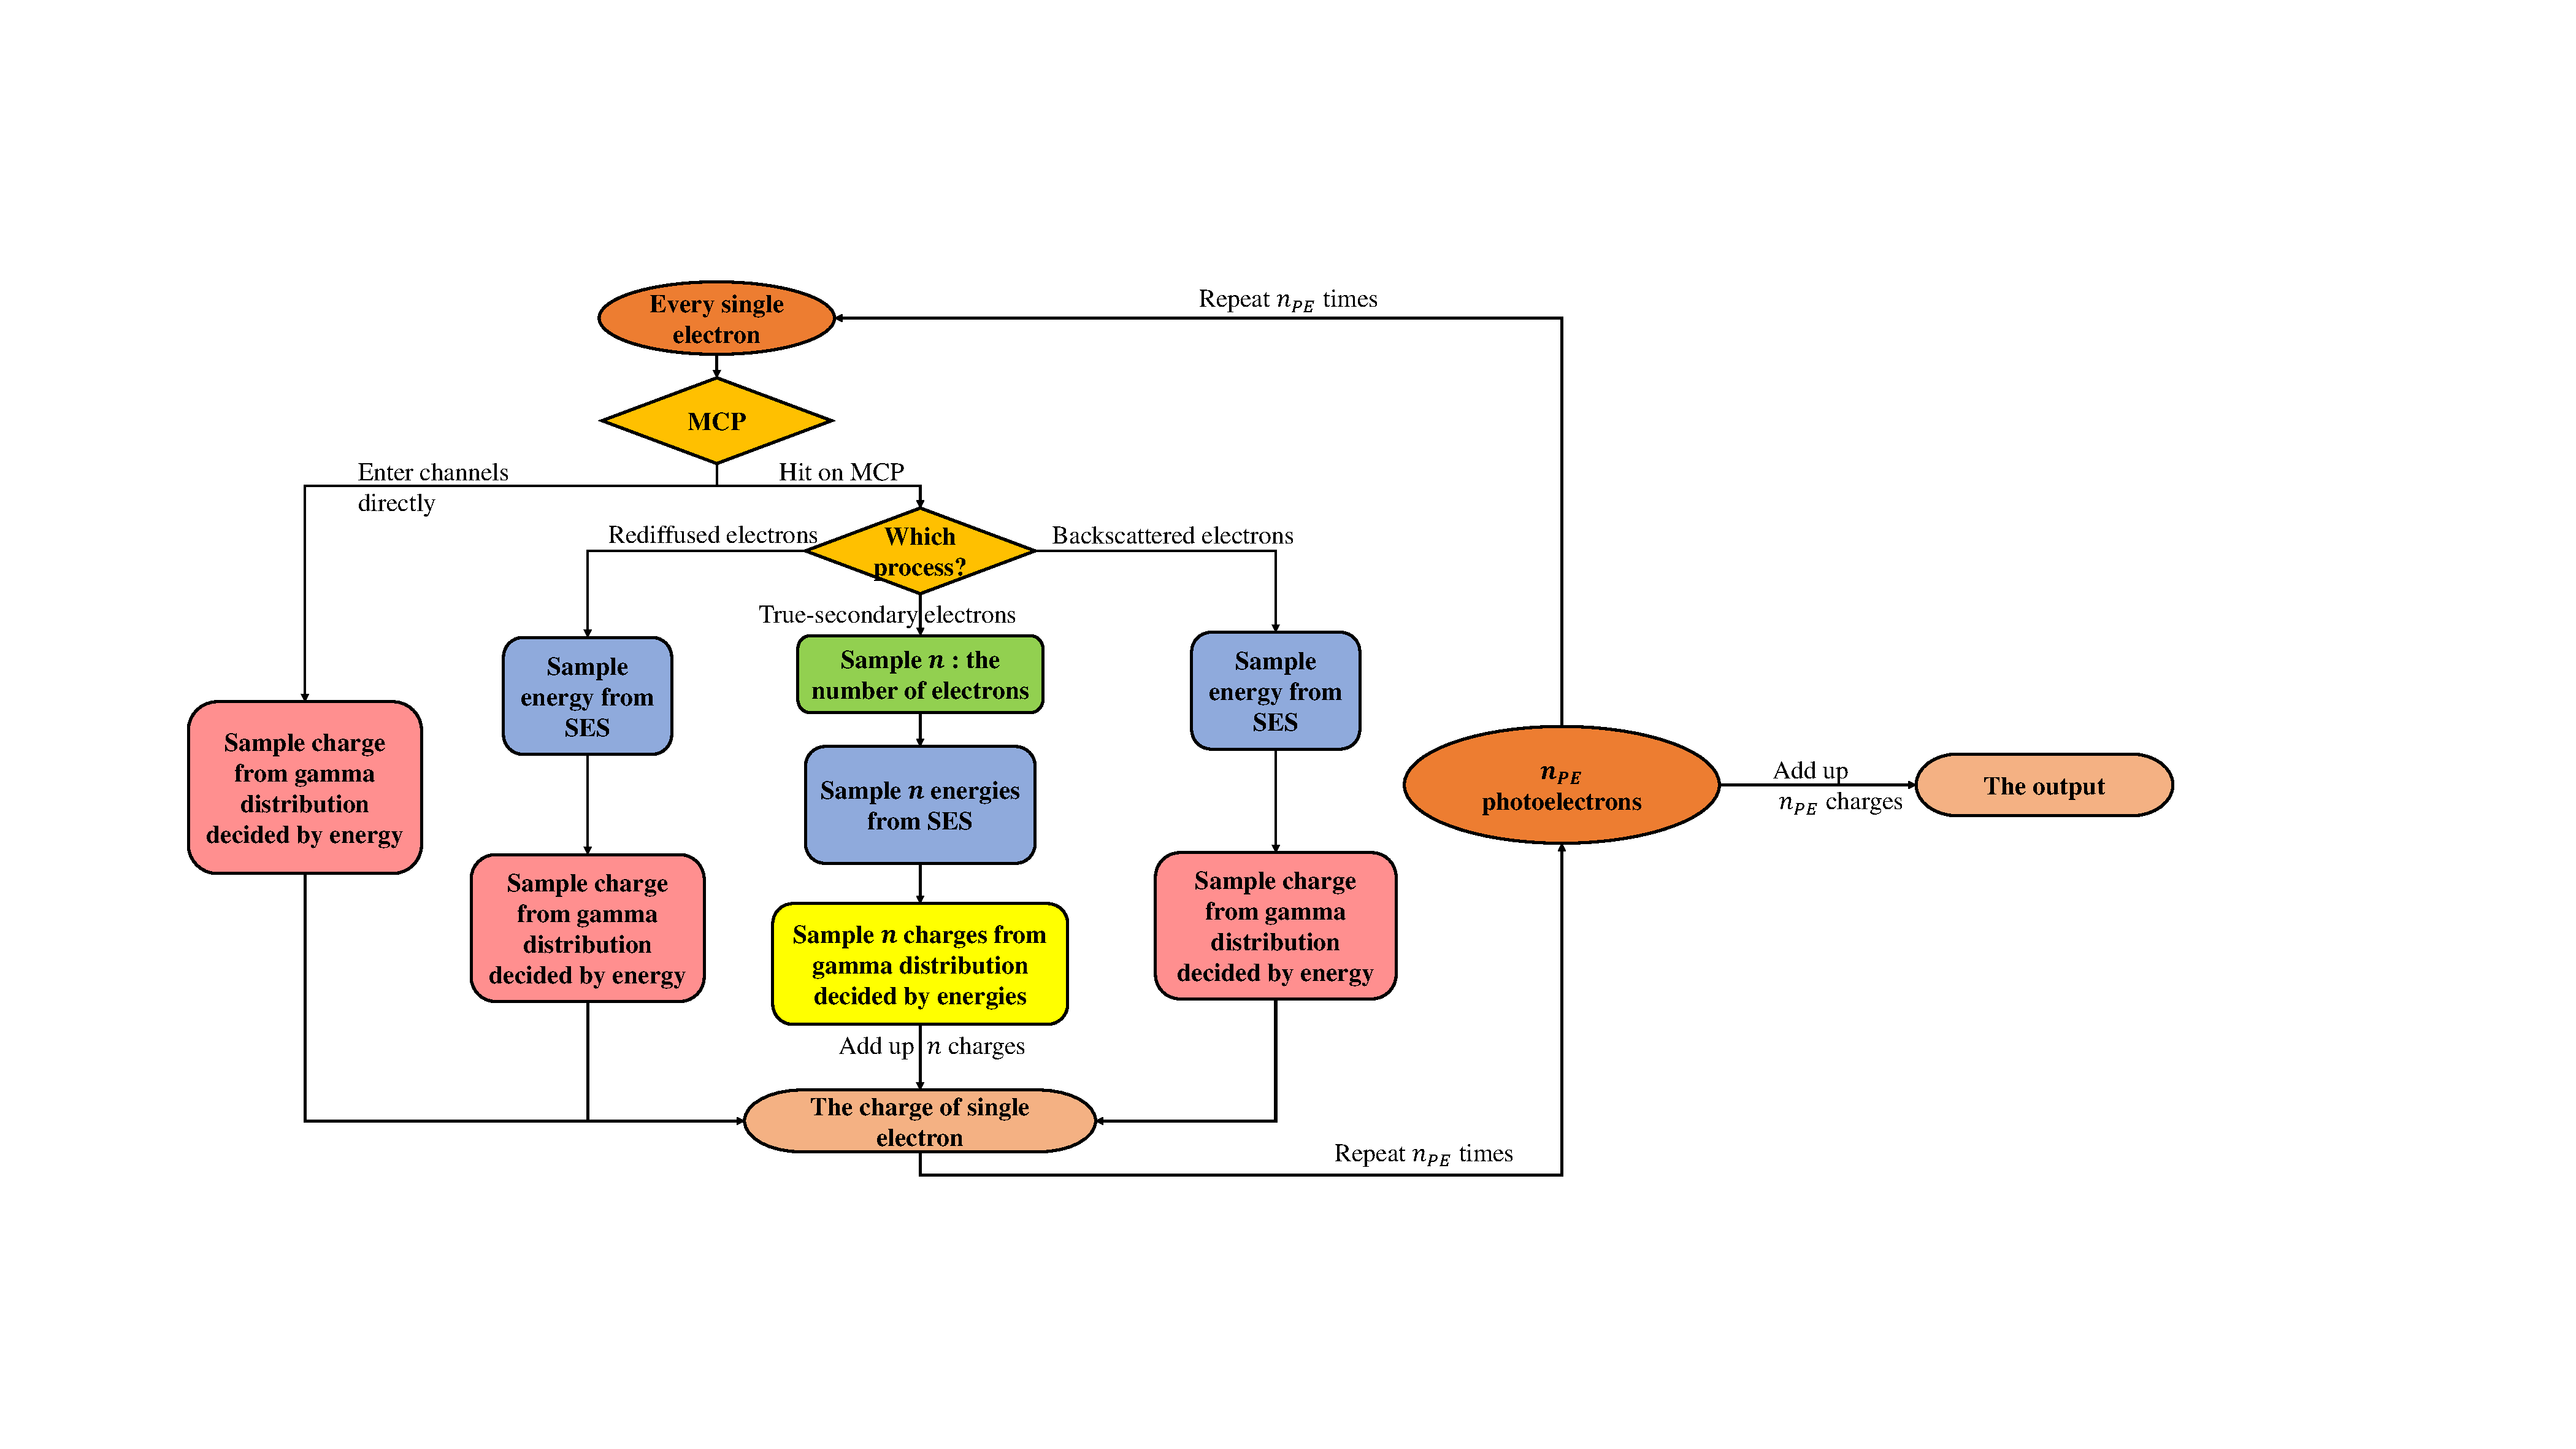
\includegraphics[width=0.95\linewidth]{pic/process.pdf}
    \caption{The procedure of Monte Carlo method for computing the SER charge spectrum.}
    \label{fig:process}
\end{figure}
Through the procedure, the charge response generated by a single electron incoming and by $n_{\mathrm{PE}}$ are calculated.
\begin{figure}[ht]
    \centering
    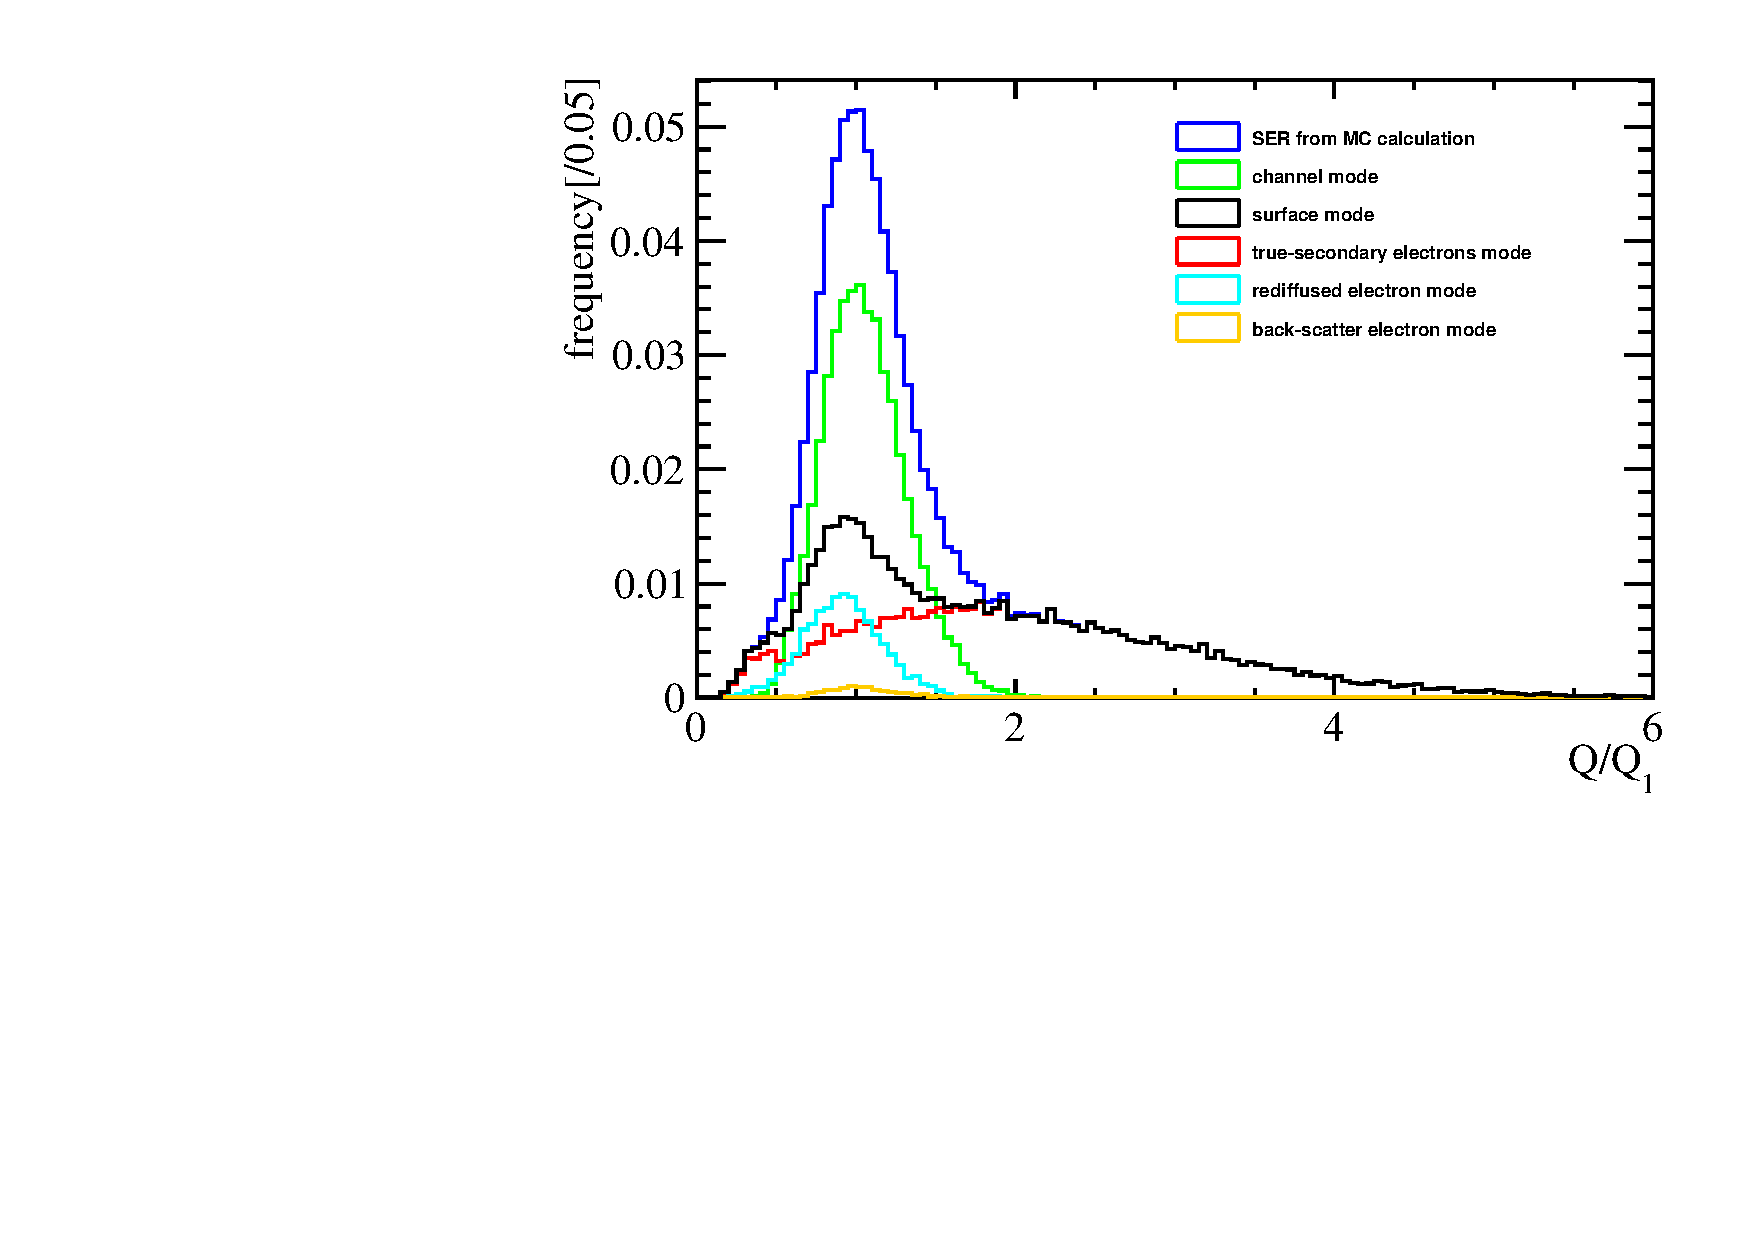
\includegraphics[width=0.6\linewidth]{pic/allmode.pdf}
    \caption{The charge distribution formed in the channel mode is concentrated around the main peak,
        while the tail portion is mainly generated by the true-secondary electrons in the surface mode.}
    \label{fig:allmode}
\end{figure}
The charge distribution of the surface mode can be divided into three components according to the Furman model,
the back-scattered electron mode defined as $Q_{\mathrm{bs}}$,
the rediffused electron mode defined as $Q_{\mathrm{rd}}$,
and the true-secondary electrons mode defined as $Q_{\mathrm{ts}}$.
\begin{equation}
    \label{eq:surface_3}
    Q_{\mathrm{surface}} = Q_{\mathrm{ts}}+Q_{\mathrm{rd}}+Q_{\mathrm{bs}}
\end{equation}

The back-scattered electron mode is predominantly distributed at the main peak,
while the rediffused electron mode exhibits a distribution in close proximity to the main peak.
These two components within the surface mode contribute to a single secondary emission electron.
There exists little difference in energy between in the channel mode and in the back-scattered electron mode
resulting in that the amplified charge is basically the same.
Due to the energy of the rediffused electron slightly lower than that in the channel mode,
the amplified charge after MCP multiplication is slightly smaller.
Therefore, the contribution of these two modes to the large charges in SER charge spectrum can be considered negligible.

In the true-secondary electrons mode, the charge can be described as Eq.~\eqref{eq:ts_all}:
\begin{equation}
    \label{eq:ts_all}
    \begin{aligned}
         & Q_{\mathrm{ts}} = \sum_{n=0}^{\infty} \sum_{i=0}^{n} Q_{\mathrm{i}}      \\
         & Q_{\mathrm{i}} \sim \varGamma  (\alpha_{\mathrm{i}}, \beta_{\mathrm{i}}) \\
         & n \sim \mathrm{\pi}(\delta_{\mathrm{ts}})
    \end{aligned}
\end{equation}
\begin{figure}[ht]
    \centering
    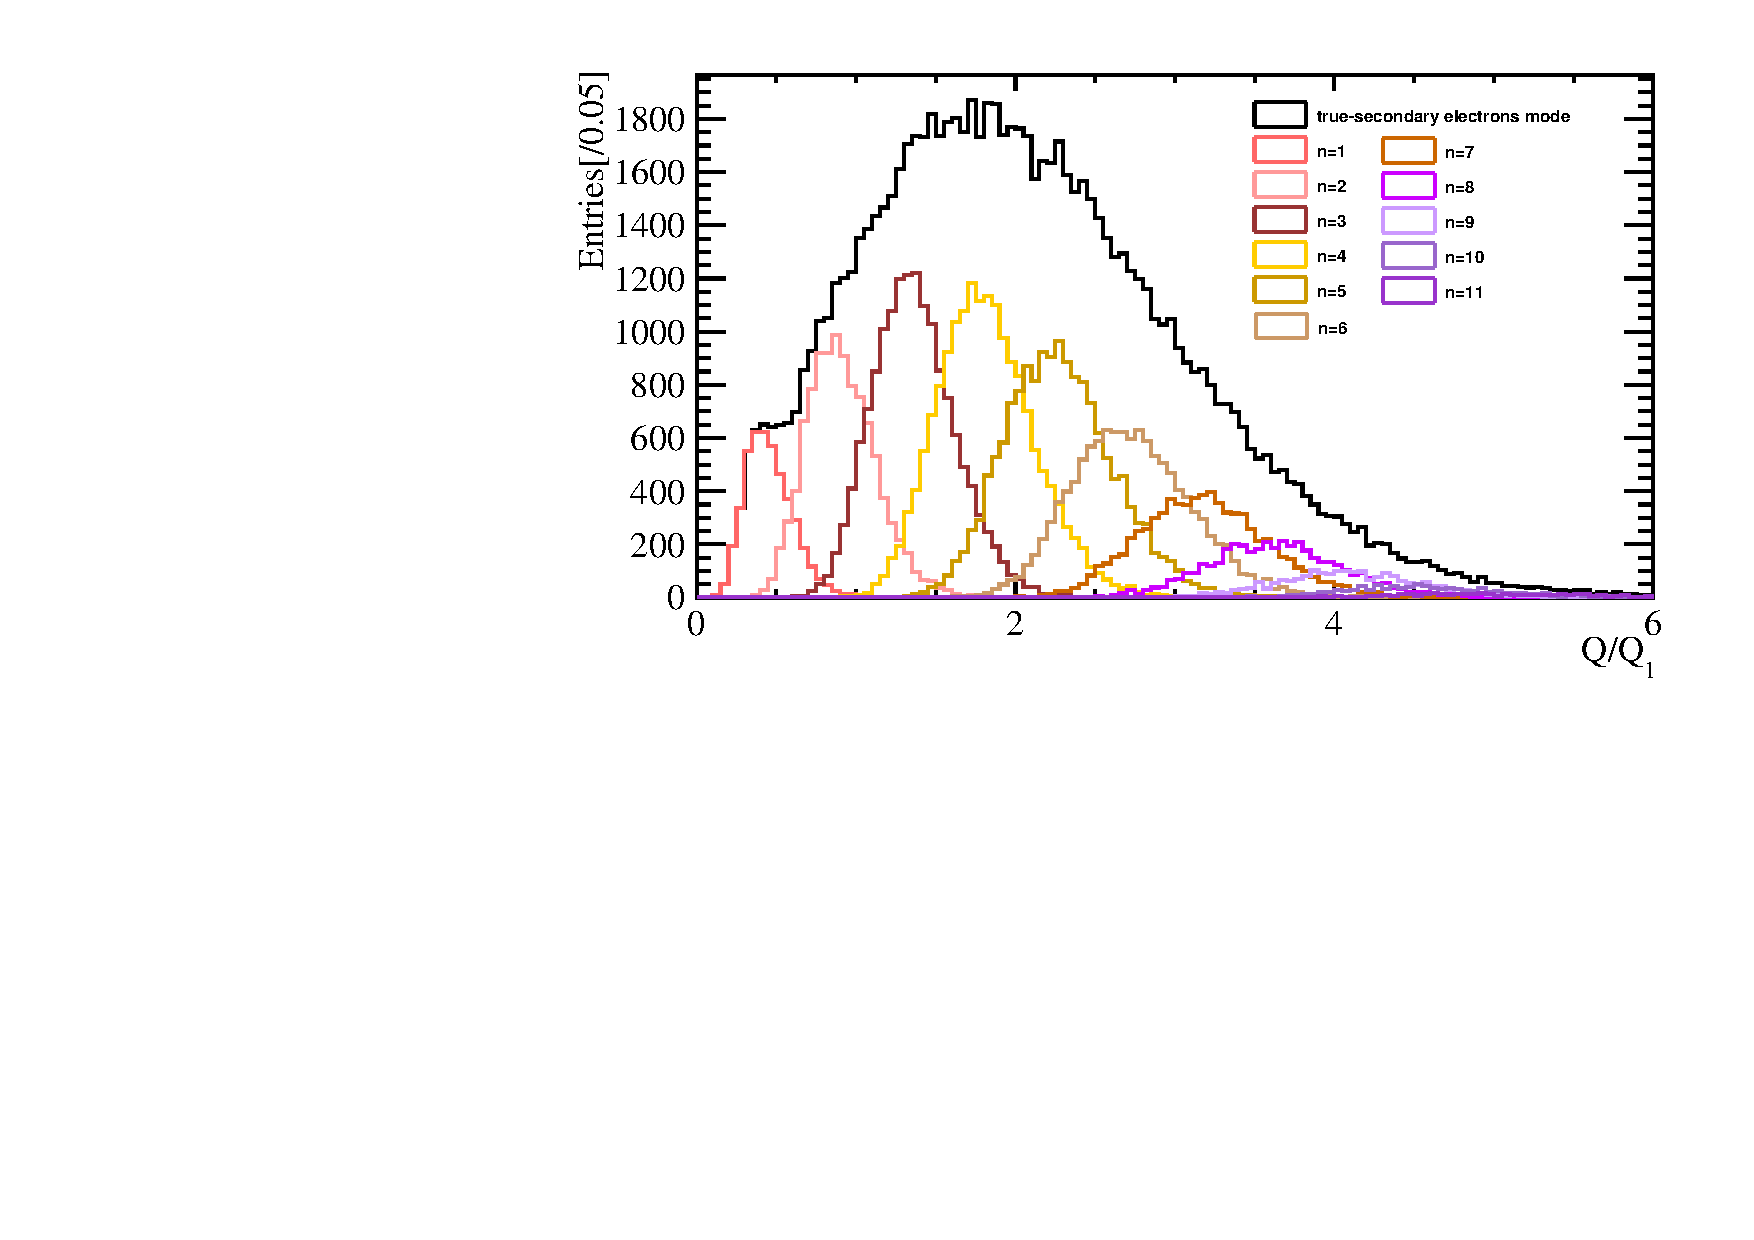
\includegraphics[width=0.6\linewidth]{pic/true_all.pdf}
    \caption{The charge distribution of true-secondary electrons mode in MC calculation when $\delta_{\mathrm{ts}}=4.5$ and $p=0.5$.
        The black histogram is the total distribution consisting of the histograms for different $n$.}\label{fig:true_n}
\end{figure}

The charge spectrum of different $n$ is shown in Fig.~\ref{fig:true_n}.
For each photoelectron in true-secondary electrons mode,
the output is the sum of the $n$ charges and the bigger $n$ is, the larger the charge is.
Due to the lower energy of the generated electrons,
the charge after each electron multiplication is smaller.
It is challenging to distinguish the multiplied charges formed at the anode,
as multiple secondary electrons are generated and enter the MCP channels simultaneously.
Their combined form results in a larger charge formation,
contributing to the "long-tail" of the SER charge spectrum.


\subsection{Tuning model with experiment data}\label{subsec:chitest}
The field $\delta_{\mathrm{ts}}$ of the true-secondary electrons and the probability $p$ in Eq.~\eqref{eq:convolution}
which have a significant impact on the SER charge distribution as shown in Fig.~\ref{fig:tsp} are selected
to generate different histograms by MC.
\begin{figure}[ht]
    \centering
    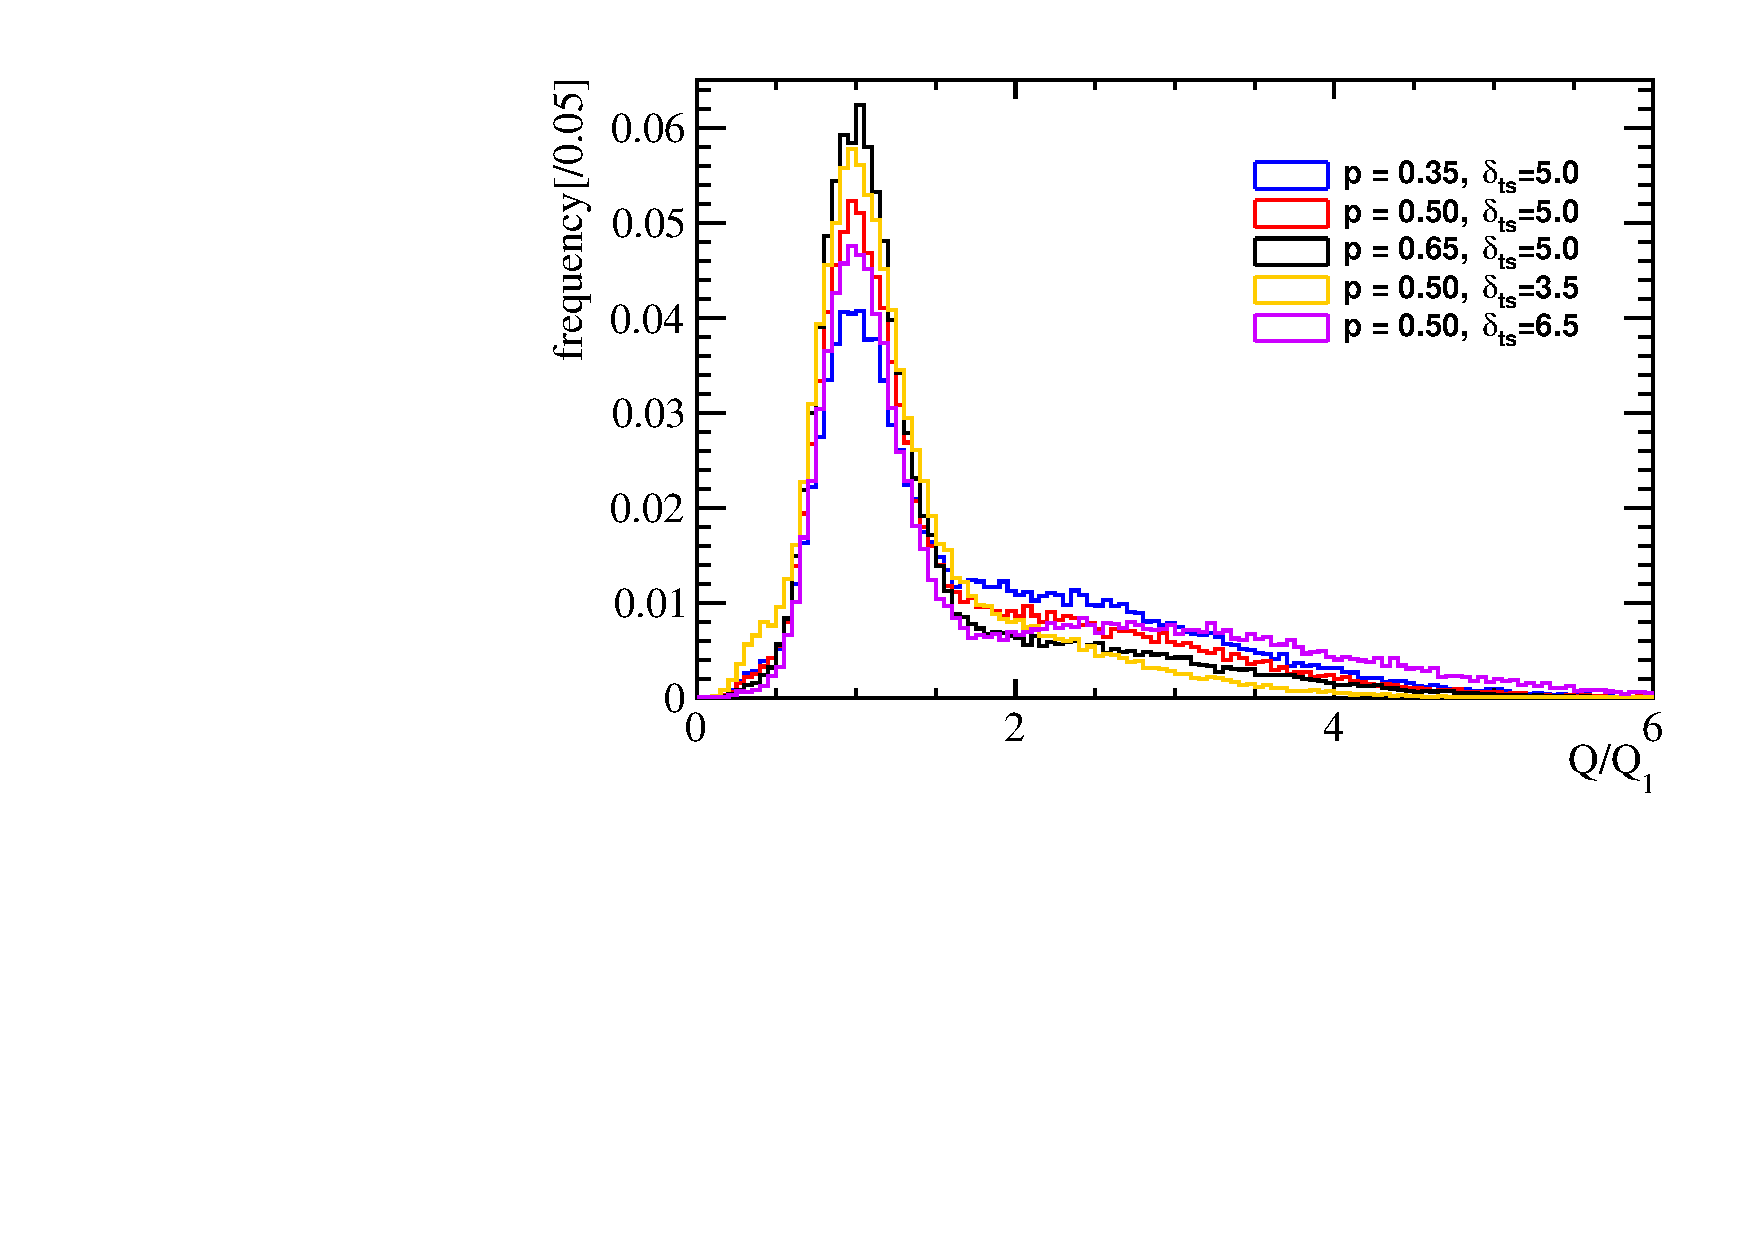
\includegraphics[width=0.6\linewidth]{pic/pts.pdf}
    \caption{The shape of SER charge spectrum from MC is influenced by $\delta_{\mathrm{ts}}$ and $p$.
        As $\delta_{\mathrm{ts}}$ increases gradually, the height of the main peak region the tail gradually becomes longer and bigger.
        As $p$ gradually increases, the height of the main peak region increases, and the tail gradually becomes narrower
    }
    \label{fig:tsp}
\end{figure}

A chi-square test is then performed between each
MC histogram and the histogram of single photoelectron charge obtained from the MCP-PMT test.
The histograms of MC and test have the same binning with the number of bins being $r$.
The entries in i-th bin are $n_{\mathrm{i}}$ and $m_{\mathrm{i}}$; total entries are
$N = \sum_{{\mathrm{i}}=1}^{r}n_{\mathrm{i}}$ and $M = \sum_{{\mathrm{i}}=1}^{r}m_{\mathrm{i}}$.
The chi-square test indicates the similarity between two histograms, with chi-square defined in Eq.~\eqref{eq:chi}~\cite{2006Comparison}.
The chi-squares between the histograms of MC and experiment data are scanned in the $p-\delta_{\mathrm{ts}}$ grid as shown in Fig.~\ref{fig:cour}.
The distribution of the chi-square
with respect to $p$ and $\delta_{\mathrm{ts}}$ is continuous,
and a linear regression can be used to fit the relationship
between chi-square and $p$ and $\delta_{\mathrm{ts}}$~\cite{oh2013introduction}.
For each MCP-PMT, the parameters corresponding to the minimum chi-square value are selected as the result.
The confidence interval for the parameters can be determined accordingly
with a confidence level of 68.3\%~\cite{cowan1997statistical}.
\begin{equation}
    \label{eq:chi}
    \begin{aligned}
         & \chi^2_{(r-1)}=\sum_{i=1}^r \frac{\left(n_{\mathrm{i}}-N \hat{k}_{\mathrm{i}}\right)^2}{N \hat{k}_{\mathrm{i}}}+\sum_{i=1}^r
        \frac{\left(m_{\mathrm{i}}-M \hat{k}_{\mathrm{i}}\right)^2}{M \hat{k}_{\mathrm{i}}}=\frac{1}{M N} \sum_{i=1}^r
        \frac{\left(M n_{\mathrm{i}}-N m_{\mathrm{i}}\right)^2}{n_{\mathrm{i}}+m_{\mathrm{i}}}                                          \\
         & \hat{k}_{\mathrm{i}}=\frac{n_{\mathrm{i}}+m_{\mathrm{i}}}{N+M}
    \end{aligned}
\end{equation}

\begin{figure}[ht]
    \centering
    \begin{subfigure}{0.47\textwidth}
        \centering
        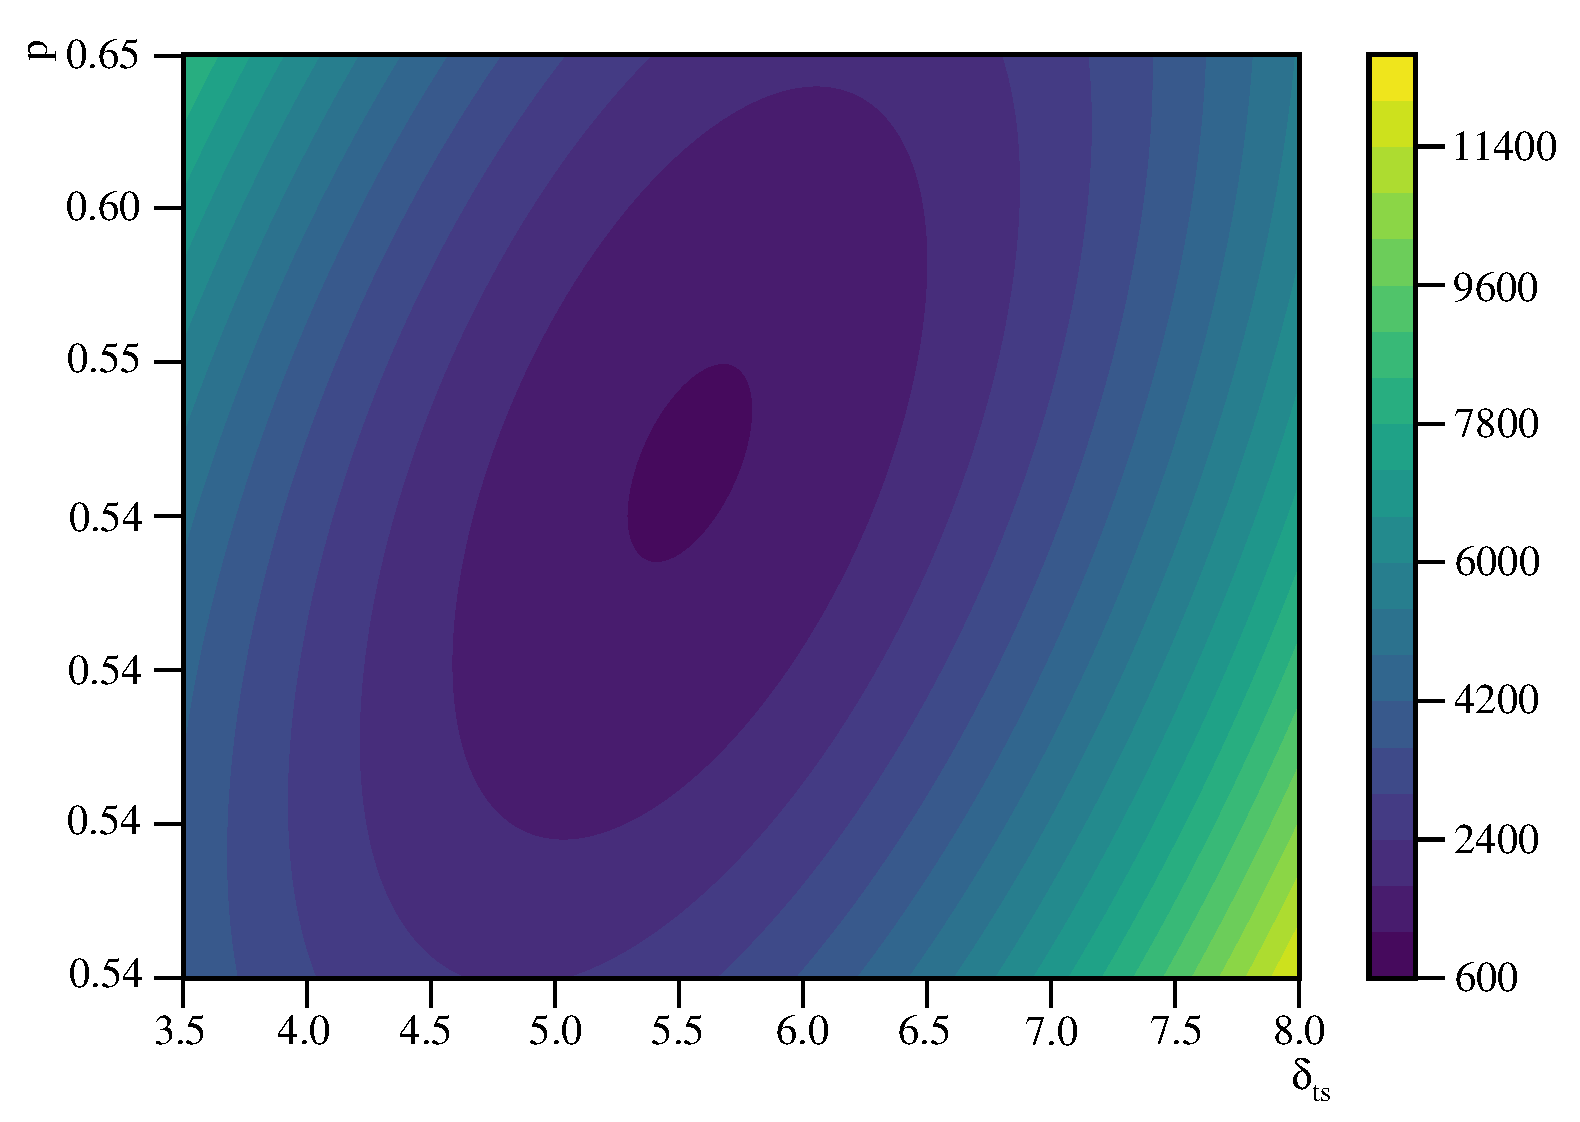
\includegraphics[height=5cm]{pic/cour.pdf}
        \caption{}
        \label{fig:cour}
    \end{subfigure}
    \hfill
    \begin{subfigure}{0.47\textwidth}
        \centering
        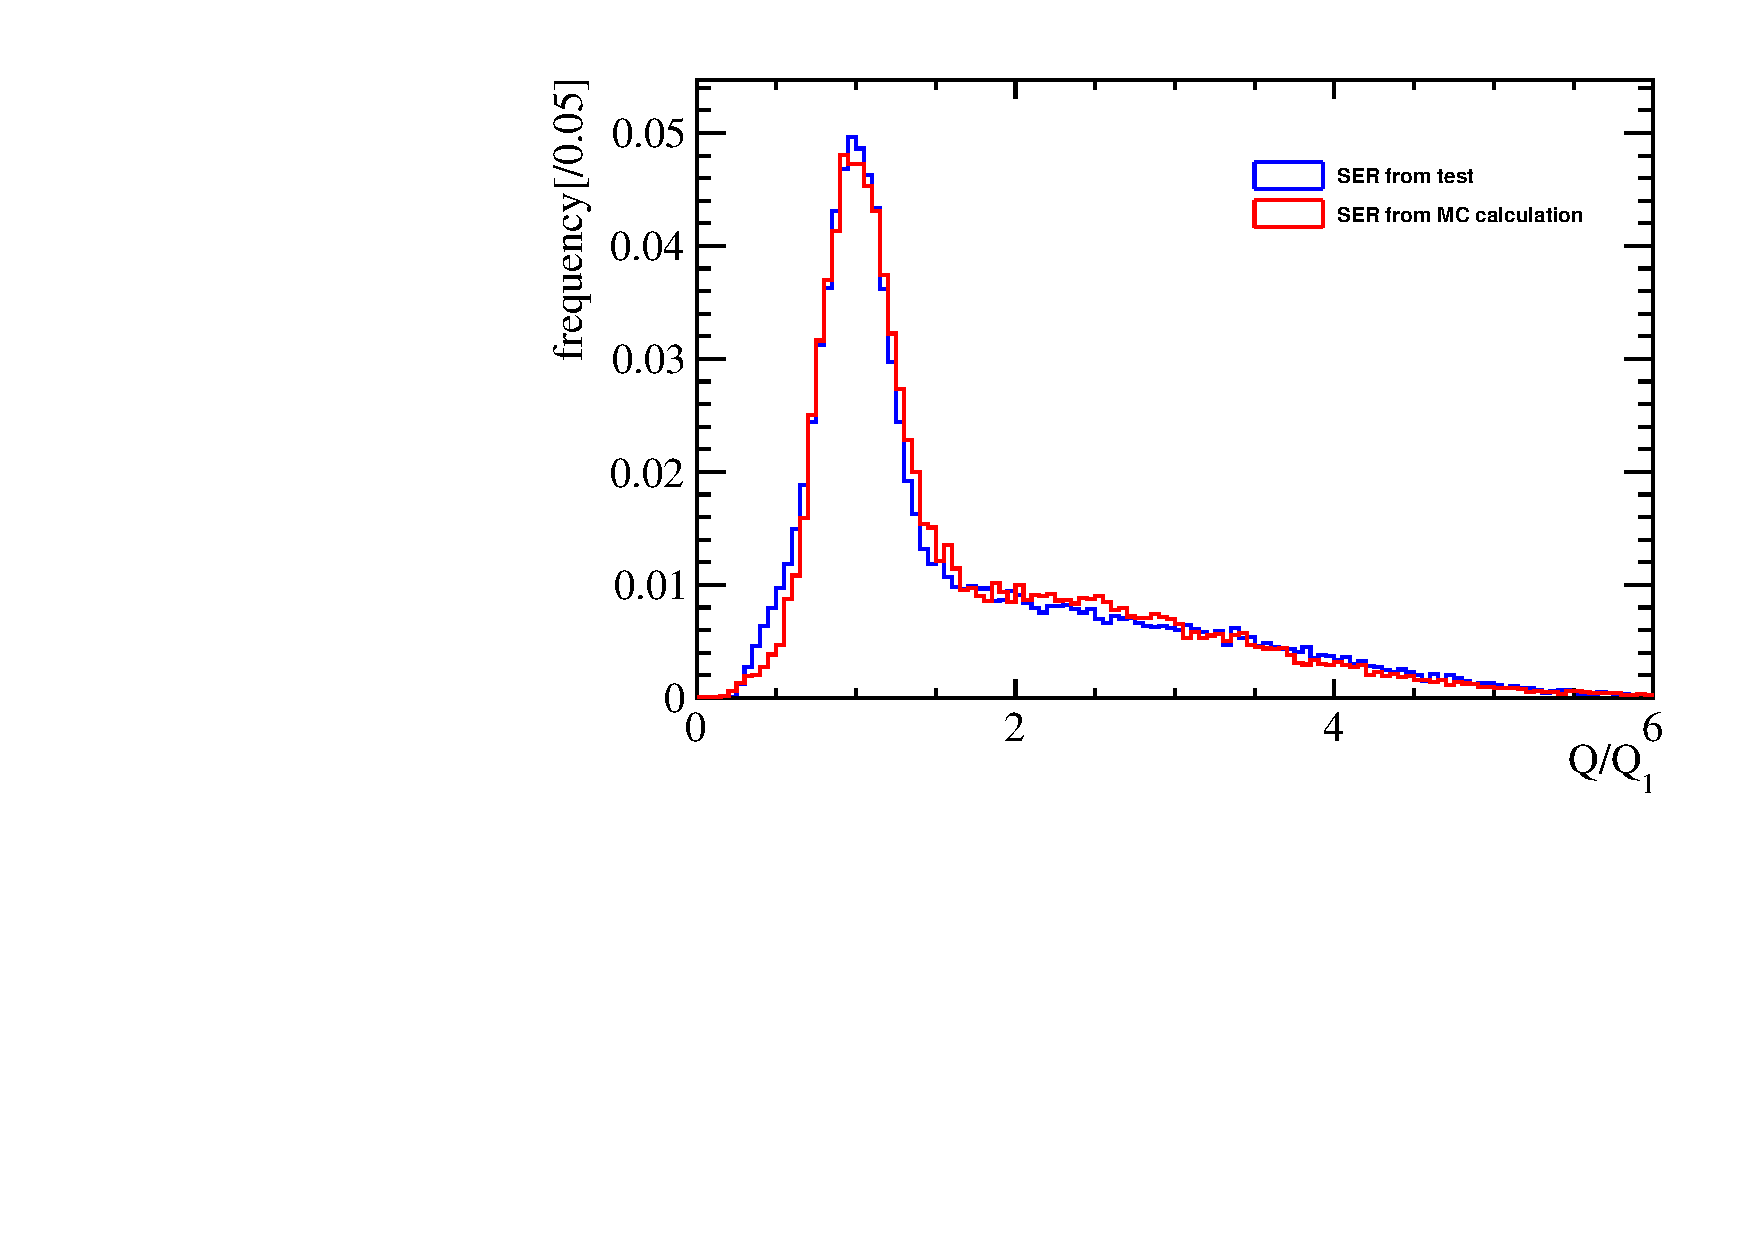
\includegraphics[height=5cm]{pic/hist.pdf}
        \caption{}
        \label{fig:hist}
    \end{subfigure}
    \caption{The plot~\subref{fig:cour} is the contour plot of the chi-square test, with $p$ and $\delta_{\mathrm{ts}}$ as parameters
        and the chi-square values as the height.
        The plot~\subref{fig:hist} is an example of the MC histogram~(the red line) and the histogram from test~(the blue line).
    }
    \label{fig:chi}
\end{figure}

The scatter plot of the $\delta_{\mathrm{ts}}$ and $p$ of 9 MCP-PMTs at the minimum
chi-square is shown in Fig.~\ref{fig:true_p}. The mean of $\delta_{\mathrm{ts}}$
is 5.98 and of $p$ is 0.531, which means that on average,
0.531 electrons directly enter the channel of the MCP.
For each electron incident on the surface of the MCP,
5.98 true-secondary electrons are multiplied.
\begin{figure}[H]
    \centering
    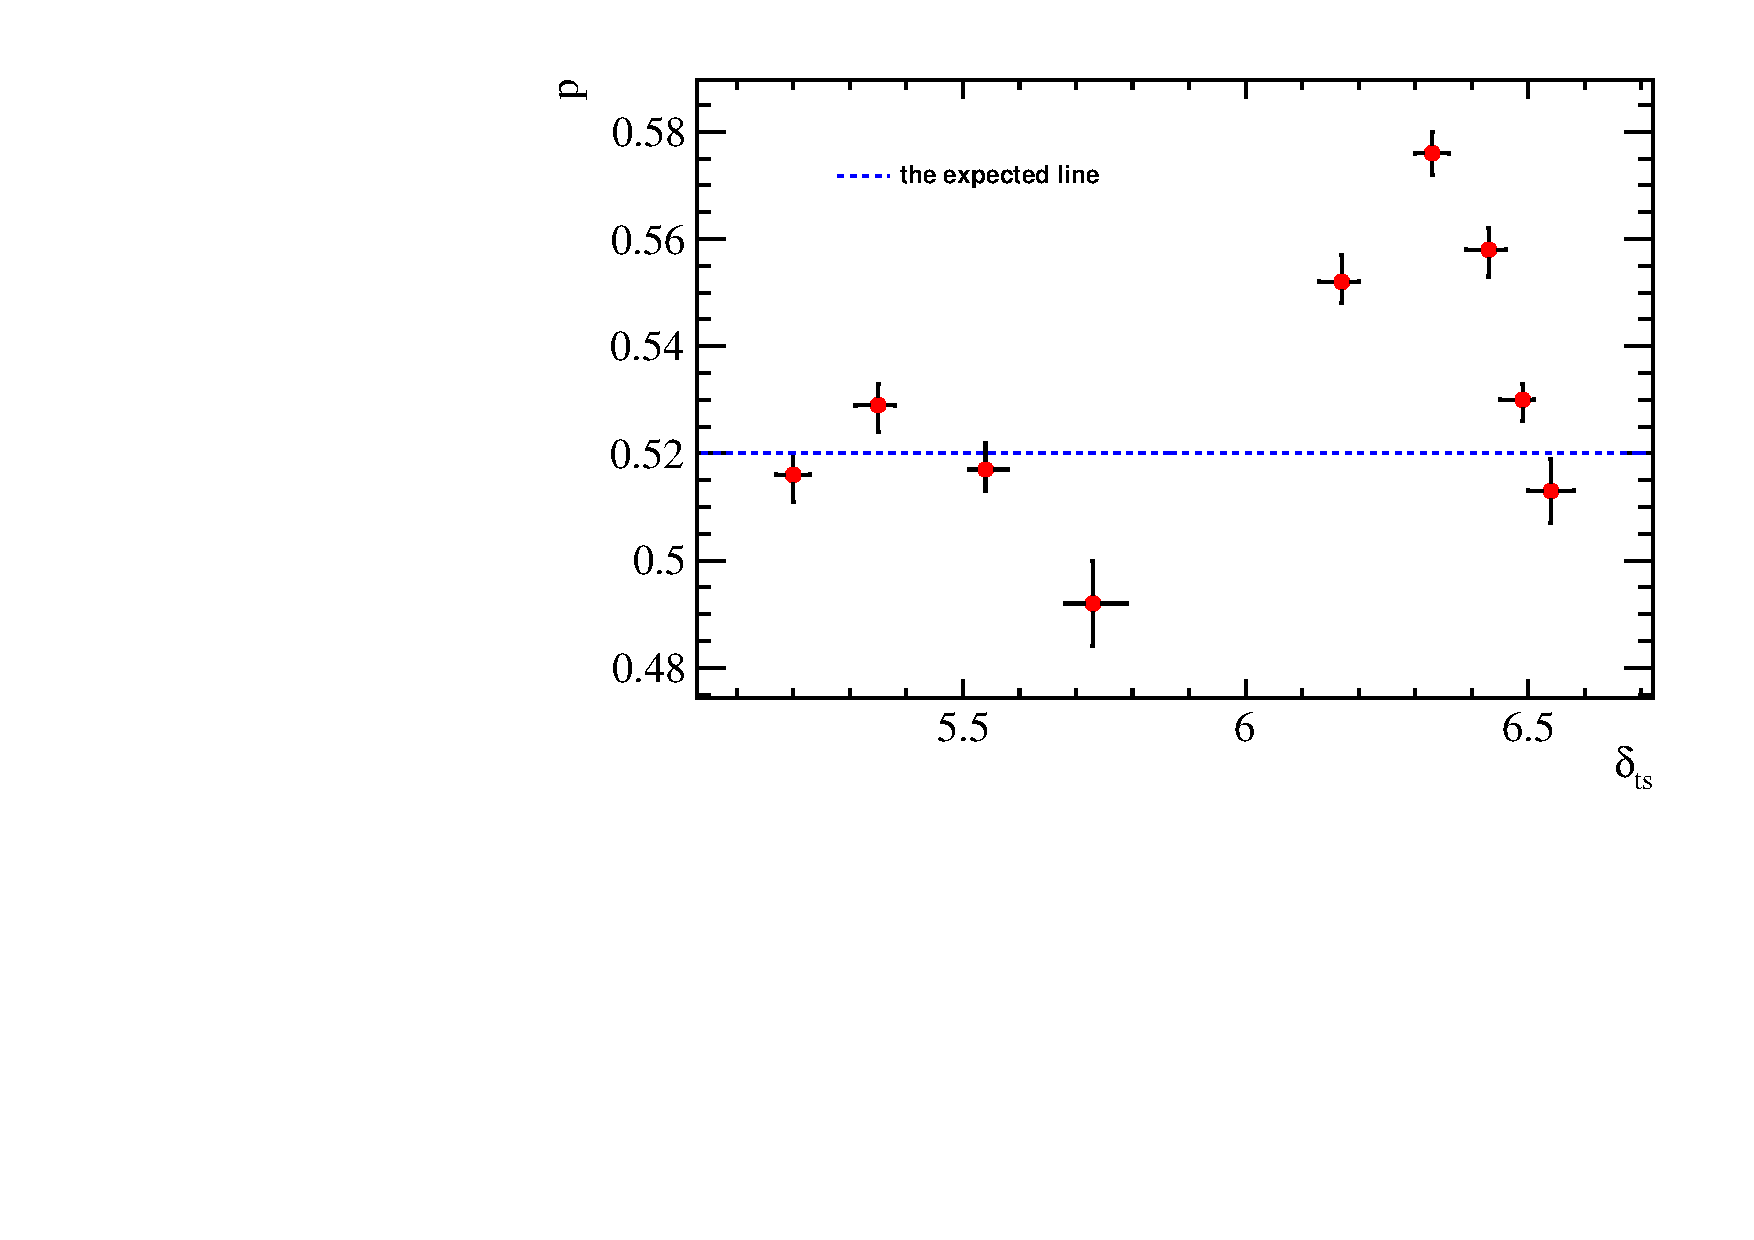
\includegraphics[width=0.6\textwidth]{pic/true_p.pdf}
    \caption{When convolving with 9 MCP-PMTs,
        the distribution of $\delta_{\mathrm{ts}}$ and $p$ at the minimum chi-square
        occurs. The blue dashed line shows the expected $p$.}
    \label{fig:true_p}
\end{figure}

The MCP open area fraction of the MCP-PMT used in JNE is around 65\%
which is significantly higher than the result of the chi-squared test.
Lin Chen. pointed out that there is the electrostatic lens effect at the MCP channel entrances
reasulting in the ratio of photoelectrons entering MCP channels
being smaller than the open area fraction.
When photoelectrons come from the top of the MCP-PMT,
the proportion of the photoelectrons directly entering the MCP channels is around 60\%
while MCP open area fraction is 74.9\%~\cite{2016Optimization}.
This ratio is extended to the MCP-PMT used in JNE,
the stronger electric field brought by smaller PMT size is considered,
and the open area fraction is smaller, $52\%\pm8\%$ is acceptable and the result of chi-square test is reasonable.

\section{Statistical model of SER for MCP-PMT}\label{sec:model}
The MC calculation in Sec.~\ref{sec:convolution} can be expressed using mathematical equations
and abstracted into a model describing the charge of the MCP-PMT shown as Eq.~\eqref{eq:gammaTweedie}:
\begin{equation}
    \label{eq:gammaTweedie}
    \begin{aligned}
        Q_{\mathrm{MCP-PMT}} & = p\times Q_{\mathrm{channel}} + (1-p)\times Q_{\mathrm{surface}}                      \\
                             & = p\times Q_{\mathrm{channel}}+(1-p)\times (p_{\mathrm{ts}}
        \times Q_{\mathrm{ts}}+p_{\mathrm{rd}}\times Q_{\mathrm{rd}}+p_{\mathrm{bs}}\times Q_{\mathrm{bs}})           \\
                             & = p_0\times Q_{\mathrm{peak}} + (1-p_0)Q_{\mathrm{ts}}                                 \\
                             & = p_0\times Q_{\mathrm{peak}} + (1-p_0)\sum_{n=0}^{\infty}\sum_{i=0}^{n}Q_{\mathrm{i}}
    \end{aligned}
\end{equation}

In Eq.~\eqref{eq:gammaTweedie}, the spectra of $Q_{\mathrm{channel}}$, $Q_{\mathrm{rd}}$ and $Q_{\mathrm{bs}}$ are similar and
merged into a new component defined as $Q_{\mathrm{peak}}$ which follows Gamma distribution.
The other component is just $Q_{\mathrm{ts}}$ which is the reason
for the generation of the large charges in SER charge spectrum.

In MC calculation, $Q_{\mathrm{i}}$ follows Gamma distribution $\varGamma(\alpha_{\mathrm{i}},\beta_{\mathrm{i}})$ determined by $E_{\mathrm{i}}$,
the energy of true-secondary electrons which satisfies $\sum_i^nE_{\mathrm{i}}<E_0$.
Due to $n$ following the Poisson distribution with a mean between 5 and 7,
the probability of $n$ exceeding 10 is negligible.
At the same time, the total energy of the electrons is 650,
which is tens of times the energy of the true-secondary electrons in the SES.
The effect of $n$ on $E_{\mathrm{i}}$ can be ingnored
and all the energies of true-secondary electrons follow the same distribution.
As a result, the charge response of every true-secondary electron
can be treated indistinguishable regardless of the value of $n$ shown in Fig.~\ref{fig:single_pe}.
A Gamma distribution is deployed to fit the charge response of single true-secondary electron
shown in Fig.~\ref{fig:single_fit} and obtains a sufficiently good fit.

\begin{figure}[ht]
    \centering
    \begin{subfigure}{0.45\textwidth}
        \centering
        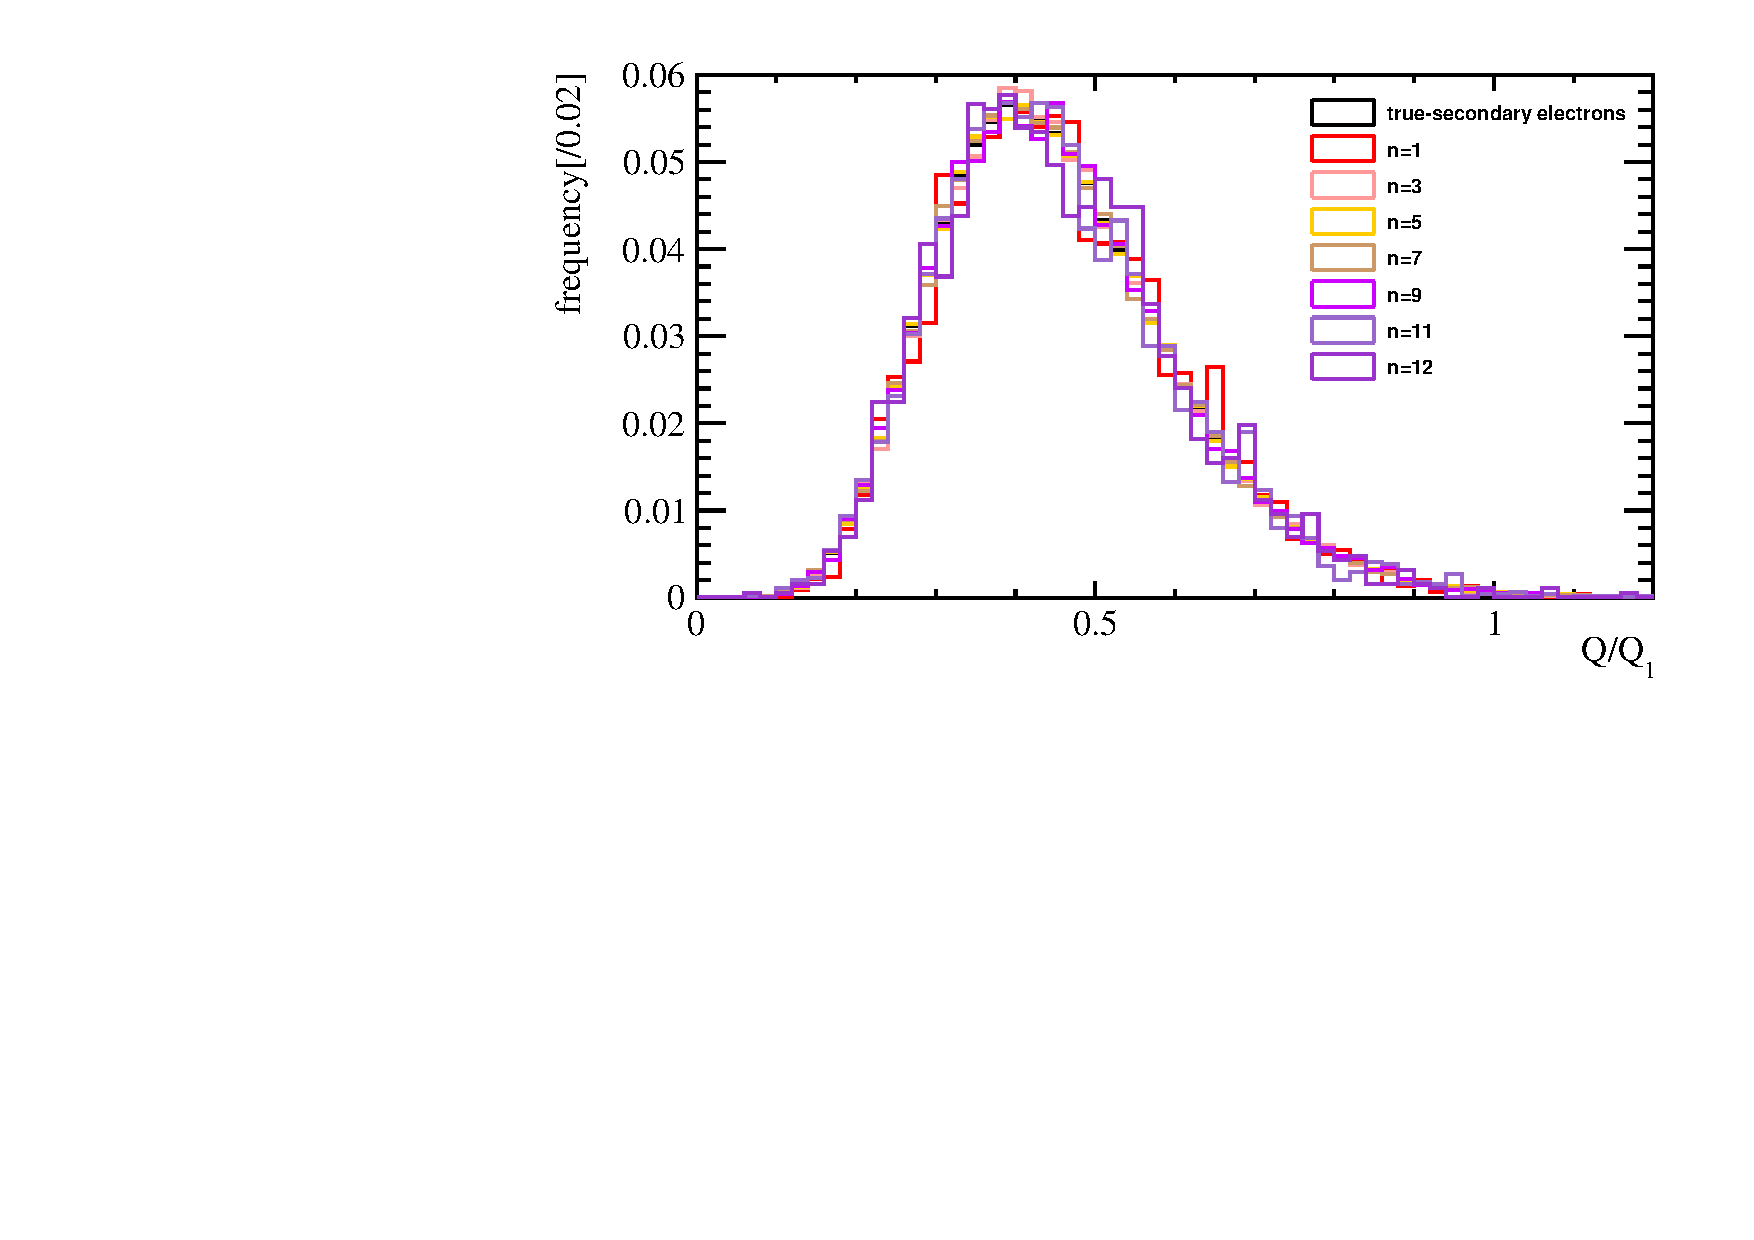
\includegraphics[width=\linewidth]{pic/single_pecharge.pdf}
        \caption{}
        \label{fig:single_pe}
    \end{subfigure}
    \hfill
    \begin{subfigure}{0.45\textwidth}
        \centering
        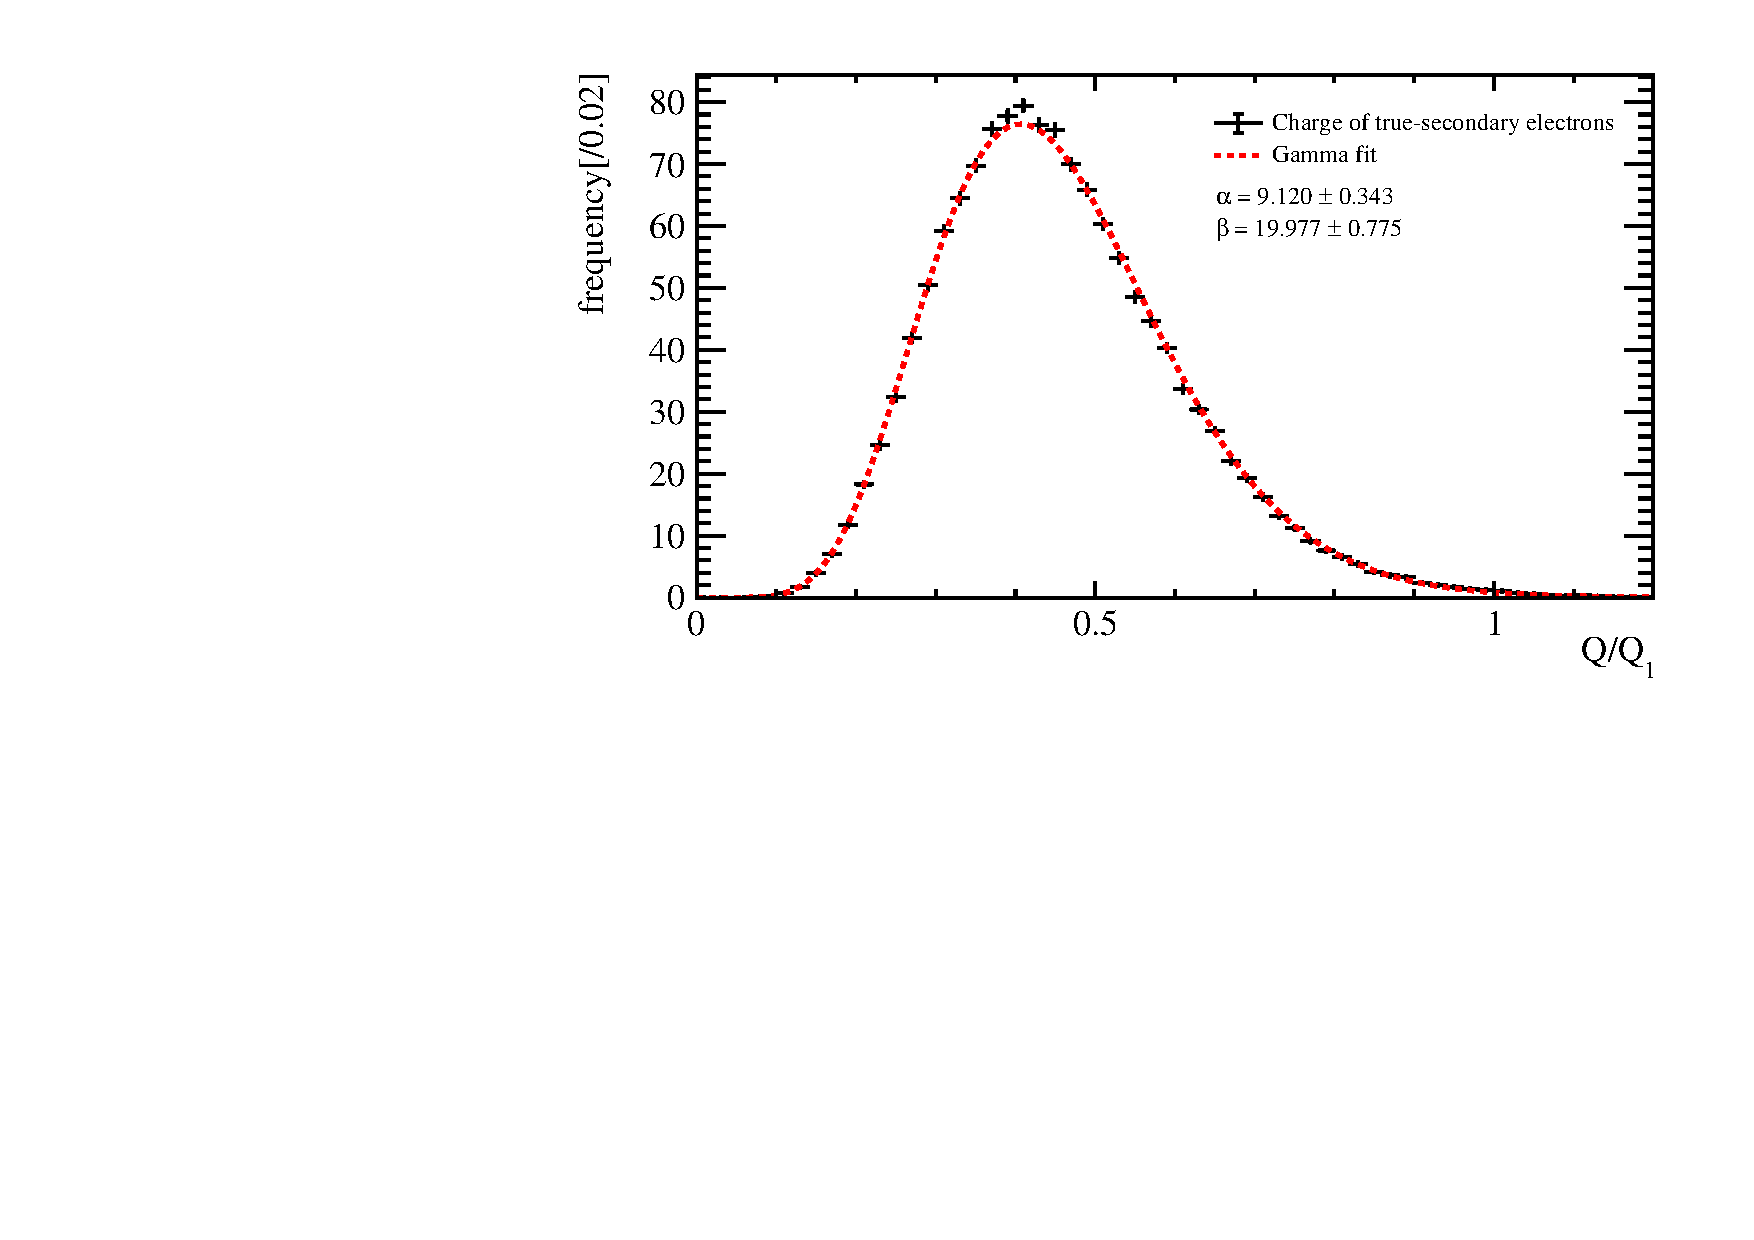
\includegraphics[width=\linewidth]{pic/singlepefit.pdf}
        \caption{}
        \label{fig:single_fit}
    \end{subfigure}
    \caption{The charge response distribution of single true-secondary electron when $n$ is different.
        The plot~\subref{fig:single_pe} shows that all the charges of true-secondary electrons follow the same distribution
        although $n$ is different.
        The plot~\subref{fig:single_fit} shows that the fitting of Gamma distribution on the charge response of single true-secondary electrons
        achieves sufficient goodness.}
    \label{fig:singlepe}
\end{figure}
$Q_{\mathrm{ts}}$ can be written as a sum of the same $n$ Gamma distributions as Eq.\eqref{eq:qts},
\begin{equation}
    \label{eq:qts}
    \begin{aligned}
         & Q_{\mathrm{ts}}=\sum_{n=0}^{\infty}\sum_{i=0}^{n}Q_{\mathrm{i}} \\
         & Q_{\mathrm{i}} \sim \varGamma(\alpha,\beta)                     \\
         & n \sim \mathrm{\pi}(\delta_{\mathrm{ts}})
    \end{aligned}
\end{equation}
which is a compound Poisson-Gamma distribution, belong to the Tweedie distribution~($\mathrm{Tw}_{\mathrm{t}}(\alpha,\beta)$)
when Tweedie power parameter $\mathrm{t}$ satisfies $1<\mathrm{t}<2$~\cite{Sen1997TheTO,1991Tweedie}.
The SER charge spectrum can be written as a Gamma-Tweedie mixture shown as Eq.~\eqref{eq:gTweedie}:
\begin{equation}
    \label{eq:gTweedie}
    \begin{aligned}
        Q_{\mathrm{MCP-PMT}} & = p_0\times Q_{\mathrm{peak}} + (1-p_0)Q_{\mathrm{ts}}                          \\
                             & Q_{\mathrm{peak}} \sim \varGamma(\alpha_{\mathrm{p}},\beta_{\mathrm{p}})        \\
                             & Q_{\mathrm{ts}} \sim \mathrm{Tw}_{\mathrm{t}}(\alpha,\beta),   1< \mathrm{t} <2
    \end{aligned}
\end{equation}


The MC calculation and chi-square test performed earlier in Sec.~\ref{sec:convolution} and \ref{subsec:chitest}
essentially constitute a joint fitting of the Gamma-Tweedie mixture.
This type of fitting is rather complex and impractical, requiring extensive computation.



\section{Discussion}\label{sec:discussion}
In experiments, it is also possible to consider incorporating the transit time distribution.
In Sec.~\ref{sec:convolution}, compared to electrons directly entering the channels of the MCP,
secondary electrons undergo a process of moving away from the MCP
before being influenced by the electric field and returning to the MCP
which increases the transit time.
By using a testing system with extremely high time resolution,
it may be possible to observe the three types of secondary electrons.
The transit time distribution may exhibit a Gaussian peak caused by back-scattered secondary electrons after the main peak,
while rediffused secondary electrons and true-secondary electrons contribute to a Gaussian peak near the main peak.
Through fitting the charge spectrum and analyzing the transit time distribution,
it becomes possible to predict the yields of the three types of secondary emission more accurately.
Certainly, $\delta_{\mathrm{ts}}$ in this study is actually the product
of the real SEY and the collection efficiency of the MCP for secondary electrons,
and can be understood as the effective true-secondary emission yield.

By the Monte Carlo simulation,
we propose the use of the Gamma-Tweedie mixture to describe the SER charge spectrum of the MCP-PMT.
While the model is designed for the MCP-PMT, it can be extended to the Dynode-PMT as well,
with the proportion $p_0$ being nearly 0
while considering only one photonelectron hitting the first dynode.
The first dynode is regarded as the MCP upper surface,
the other dynodes are collectively considered as the MCP channels.
However, no photoelectron enters the "channels" directly.
In the future, it is possible to develop calibration methods specifically for this type of MCP-PMT
to fully utilize its performance.

\section{Conclusion}\label{sec:conclusion}
ALD-coated MCP-PMTs have the higher CE,
while cause the large charges in SER charge spectrum shown in Fig.~\ref{fig:spe_sreal}.
An explanation based on the Furman secondary emission model and a voltage-division experiment are proposed.
Through innovative design utilizing a dual high-voltage circuit in voltage-division experiment,
the measurement of the gain response of MCP to electrons with different energies is achieved.
Photoelectrons hitting the upper surface of MCP generate multiple true-secondary electrons entering the channels,
which is the reason for the large charges in the SER charge spectrum of MCP-PMT.

By using the Monte Carlo method, the calculation of the SER charge spectrum of MCP-PMT has been achieved.
By performing the chi-square test, the yield of true-secondary electrons can be predicted
which is the first study on the phenomenon of SEE in pulse mode.
After conducting the chi-square test on 9 PMTs, the predicted yield is around 5.98.
Based on the explanation, a Gamma-Tweedie mixture which is a new model for the SER charge spectrum of MCP-PMT has been proposed.


\section{Acknowledgments}
Special thanks to North Night Vision Science \& Technology (Nanjing) Research Institute Co. Ltd. (NNVT)
for providing all the PMTs and the voltage dividers we need.
Also, we would like to thank Yiqi Liu, Jiashen Tao, Chuang Xu, Xin Wang and others for their assistance in the experiment,
as well as Yuyi Wang for help with data analysis. Their support and assistance have been crucial to this study.
This work is supported in part by the National Natural Science Foundation of China (12127808),
National key research and development program of China~(Grant no. 2023YFC3107400),
and the Key Laboratory of Particle \& Radiation Imaging (Tsinghua University).

\bibliographystyle{plain}
\bibliography{ref}
\end{document}
